\documentclass[12pt,PhD]{Thesis}



% ******** vmargin settings *********
\usepackage{vmargin} %This give you full control over the used page area, it maybe not the idea method in Latex to do so, but I wanted to reduce to amount of white space on the page
\setpapersize{A4}
%\setmargins{3.5cm}%			%linker Rand, left edge
%	  {1cm}%     %oberer Rand, top edge
%           {14.7cm}%		%Textbreite, text width
%           {23.42cm}%   %Texthoehe, text hight
%           {14pt}%			%Kopfzeilenhöhe, header hight
%           {1cm}%   	  %Kopfzeilenabstand, header distance
%           {0pt}%				%Fußzeilenhoehe footer hight
%           {2cm}%    	  %Fusszeilenabstand, footer distance   


%Defining text font profile
\usepackage{t1enc} % as usual




\usepackage[latin1]{inputenc} % as usual
\usepackage{times}	
\usepackage{mathcomp, subfigure}
\usepackage{amsmath}
\usepackage[pdftex]{graphicx}

\pagestyle{plain}
%\renewcommand{\topfraction}{0.99}
%\renewcommand{\bottomfraction}{0.99}
%\renewcommand{\textfraction}{0}


\dept{School of Physics and Astronomy}
\submitdate{2011}

\begin{document}
%Plan
%
\title{Measurements and Simulations of Impedance Reduction Techniques in Particle Accelerators}
\author{Hugo Alistair Day}
\principaladviser{Dr. Roger Jones}


\beforeabstract
\prefacesection{Abstract}
A review of the first two years of study are presented. These topics consist of; Simulations of coaxial wire measurements of the impedance of asymmetric devices, coaxial wire measurements of ferrite kicker magnets for use in the SPS and LHC and impedance studies of a number of potential collimator upgrades for the LHC, focusing on the phase 2 secondary collimators for the LHC. Also disucssed is future work towards completion of the PhD and a timetable of writing to ensure timely completion.
\afterabstract
\afterpreface


\tableofcontents

% What is new in the thesis:
% Wire measurements of asymmetric structures
% LMCI with SC and BB impedances - reconstructing Kell-Schnell diagram
% Simulations of wire measurements of structures
% Simulations of large structures (3m of magnets/kicker magnets)
%
%
%



\chapter{Introduction}
\section{TCTP Impedance Studies}

As part of the ongoing collimation upgrade in the LHC, several advances in the LHC design have been proposed. These are as follows:

\begin{enumerate}
\item{For the reasons given in Sec.~\ref{sec:phase-2-col-mat}, the jaw material of the collimators, specifically the secondary collimators is under review in an effort to reduce the beam impedance, improve cleaning efficiency and continue the present robustness and excellent performance of the LHC collimation system.}
\item{The inclusion of on collimator BPMs. This is due to the present method of alignment of the collimators relying on investigating the beam loss patterns in the LHC as a function of collimator aperture being a very time intensive procedure due to the inherentl slow natyure of beam loss. The use of on collimator BPMs allows a near instantaneous feedback on the position of the beam relative to the collimator jaw thus greatly increasing collimator setup time[cite setup paper gianluca/on collimator BPM paper]}
\item{A new RF system (Shown in Fig.~\ref{fig:phase-2-rf-system}) to reduce the side effects of the sliding RF contacts used in the phase 1 collimators.}
\end{enumerate}

As part of the upgrade, a series of TCTP collimators shall be installed in the LHC in replacement of a number of tertiary collimators (TCTs). In total, 8 TCTP and 1 TCSG will be added to the LHC. These collimators are in part intended to act as a test for two of these upgrades, the use of on collimator BPMs and the new RF system[cite collimators with onboard BPMs]. As part of the ongoing effort to limit increases to the LHC machine impedance (shown in Tab.~\ref{tab:lhc-impedance-budget})



\begin{table}
\caption{The impedance budgets (both transverse and longitudinal) for LHC. Taken from the LHC Design Report[cite LHC design report 2003-2004]}
\begin{center}
\begin{tabular}{c | c | c}
Beam Operation & Longitudinal $\Im{}m ( Z_{\parallel}/n )$ $( \Omega )$ & Longitudinal $\Im{}m ( Z_{\perp} )$ $( \Omega /m )$\\ \hline
Total Broadband at injection (450GeV) & 0.07 & 1.34 \\ \hline
Total Broadband at collisions with squeezed optics (7TeV) & 0.076 & 2.67 \\ \hline
\end{tabular}
\end{center}
\label{tab:lhc-impedance-budget}
\end{table}


\chapter{Wakefields and Impedance}
\section{Wakefields, Impedances and Beam Dynamics Effects}

\section{Theoretical Background of Wakefields and Impedances}

%
% Explaination of the concept of wakefields (the source and witness particle), oscillating electric fields
% induced by a charged particle. Longitudinal and Transverse wakefields

\begin{itemize}
\item{Wakes}
\begin{itemize}
\item{Introduction to the electromagnetic field of charged particle moving in free space}
\item{Field of a particle in a perfectly conducting pipe - method of image currents}
\item{Place a witness particle distance s behind source particle and deduce electric field as seen by this particle}
\item{normalise this by the source particle charge to give the wakepotential}
\item{And again by the source particle charge and current profile to acquire the loss factor}
\item{Longitudinal field predominantly}
\item{Introduce the Panowsky-Wenzel theorem covering transverse field - Transverse wakes}
\end{itemize}
\item{Impedance}
\begin{itemize}
\item{Firstly mention the commonality of frequency dependent material properties - ferrite permeability, permitivitty determined by conductivity/frequency in conductors/dielectrics/skin depth}
\item{Fourier transform of wakefield into the convolution of the beam current spectrum and the impedance}
\item{Again Panowsky-Wenzel for impedance}
\item{Discussion of the transverse impedance - in particular the general definition of an impedance (n-th order current interacting with an m-th order field)}
\item{Define dipolar/driving and quadrupolar/detuning impedance. In addition constant transverse impedance term}
\end{itemize}
\end{itemize}


\subsection{Resistive Wall Impedance}

\begin{itemize}
\item{Return to simple axisymmetric geometry concerning a finite conductivity of the wall}
\item{Derive in frequency domain - then have impedance. Give an example wakefield of a good conductor (copper), bad conductor (graphite), non-conductor (ferrite)}
\end{itemize}

\subsection{Geometric Impedance}
\begin{itemize}
\item{Derive the field pattern for a pillbox cavity - Oscillating fields with a characteristic frequency of some multiple of the lowest eigenfrequency}
\end{itemize}
\section{Examples of Effects}

\section{Example of the Effects of Wakefields}
\subsection{Beam Induced Heating}
\label{sec:beam_induced_heating}
\section{Defining and Deriving Power Loss in Circular Accelerators}
\label{sec:power_loss}

When a charged particle interacts with an impedance it losses energy to generate the resulting wakefield. This is called the parasitic loss, and is generally defined as[ref Chao/Ng]

\begin{equation}
\Delta E = -2\pi e^{2}N_{b}\int^{\infty}_{-\infty} d\omega \left| \lambda \left( \omega \right)  \right|^{2} Z_{\parallel} \left( \omega \right)
\end{equation}

where $\Delta E$ is the energy loss per pass per particle, $e$ is the charge per particle, $N_{b}$, $\omega$ the frequency, $\lambda$ the line density of the bunch and $Z_{\parallel}$ the longitudinal impedance of the object being traversed.
																
Due to the decay of the wakefields induced by this energy loss, this energy must eventually be lost to the device causing the impedance (valid below the cutoff frequency of the machine beam pipe). Therefore we can assume that the energy loss from the particles is absorbed by the surrounding structure. Summing over all particles in a bunch we can therefore obtain a sum of the energy loss;

\begin{equation}
\Delta E_{bunch} = 2\pi \left( eN_{b}   \right)^{2} \int^{\infty}_{-\infty} d\omega \left| \lambda \left( \omega \right)  \right|^{2} Z_{\parallel} \left( \omega \right)
\end{equation}

As often we must deal with machines storing multiple bunches, for these we simply multiply the energy loss per bunch by the number of stored bunches to acquire the total energy loss per passage;

\begin{equation}
\Delta E_{bunches} = 2\pi \left( eN_{b}   \right)^{2}n_{bunch} \int^{\infty}_{-\infty} d\omega \left| \lambda \left( \omega \right)  \right|^{2} Z_{\parallel} \left( \omega \right)
\end{equation}

where $n_{bunch}$ is the number of bunches in the machine. If we assume a revolution frequency $f_{rev}$ we thus get a power loss of;

\begin{align}
P_{loss}  = & \Delta E_{bunches} f_{rev}\nonumber \\  
 = & 2\pi f_{rev} \left( eN_{b}   \right)^{2}n_{bunch} \int^{\infty}_{-\infty} d\omega \left| \lambda \left( \omega \right)  \right|^{2} Z_{\parallel} \left( \omega \right) \nonumber  \\ 
 = & 2\pi f_{rev} \left( eN_{b}   \right)^{2}n_{bunch} \int^{\infty}_{-\infty} d\omega \left| \lambda \left( \omega \right)  \right|^{2} Z_{\parallel} \left( \omega \right) \nonumber \\
 = & 2\pi f_{rev} \left( eN_{b}   \right)^{2}n_{bunch} \int^{\infty}_{-\infty} d\omega \left| \lambda \left( \omega \right)  \right|^{2} \left( \Re{}e \left( Z_{\parallel} \left( \omega\right) + \Im{}m Z_{\parallel} \left( \omega\right) \right) \right).
\end{align}
 
As $\Re{}e\left(Z_{\parallel} \left( \omega\right)\right)$ is an even function and $\Im{}m\left(Z_{\parallel} \left( \omega\right)\right)$ is an odd function, we see that

\begin{equation}
P_{loss}   =  \omega_{rev} \left( eN_{b}   \right)^{2}n_{bunch} \int^{\infty}_{0} 2 d\omega \left| \lambda \left( \omega \right)  \right| ^{2}  \Re{}e \left( Z_{\parallel} \left( \omega\right)  \right).
\label{eqn:power_loss_omega}
\end{equation}

Next we make a change of the variable of integration $\omega = n_{bunch}\omega_{rev}$;

\begin{equation}
P_{loss}   =  \omega_{rev} \left( eN_{b}   \right)^{2}n_{bunch}^{2} \int^{\infty}_{0} 2 d\omega_{rev} \left| \lambda \left( \omega_{rev}n_{bunch} \right)  \right|^{2}  \Re{}e \left( Z_{\parallel} \left( \omega_{rev}n_{bunch}\right)  \right).
\end{equation}

We can subsequently change to a sum formalism to obtain

\begin{equation}
P_{loss} = \left( \omega_{rev}eN_{b}n_{bunch}  \right)^{2} \displaystyle\sum\limits_{p = 0}^{\infty} \left( 2 \left| \lambda \left(p \omega_{rev}n_{bunch} \right)  \right|^{2}  \Re{}e \left( Z_{\parallel} \left(p \omega_{rev}n_{bunch}\right) \right) \right) \label{ean:heating-gen}
\end{equation}

where $\omega_{0} = 2\pi f_{0}$, $f_{0} = \frac{1}{\tau_{b}}$ and $\tau_{b}$ is the bunch spacing.

\section{Longitudinal Beam Profiles}

As shown by the derivations in Section~\ref{sec:power_loss}, asides from the longitudinal impedance of the device under consideration the longitudinal profile of the circulating bunches also contributes to the power loss in the machine. In past works it has generally been assumed that bunches in accelerators have a Gaussian profile [ref Sacherer/Grudiev/Laclare](seen in Eqn.~\ref{eqn:gauss}, where $4\sigma_{z} = t_{b}$, $t_{b}$ is the bunch length) when approaching the analytical treatment of beam instabilities, both single-bunch and multi-bunch. Recent measurements of the power spectrum of particle beams, especially in the LHC [ref theo/phillipe] have shown characteristics that the Gaussian profile does not predict, for example the high frequency secondary peak as seen in Fig.~\ref{fig:measured_gauss}. To make more realistic predictions of heat loss due to beam impedance in the machine it is thus necessary to find bunch profiles which reproduce this behaviour.

\begin{equation}
\lambda \left( t \right) = e^{\frac{-t^{2}}{2\sigma^{2}}}
\label{eqn:gauss}
\end{equation}

\begin{figure}
\subfigure[]{
\includegraphics[width=0.45\textwidth]{Wakefields_and_Impedances/figures/beam_spectra_power_gauss_meas_12ns.pdf}
\label{fig:gauss_meas_freq}
}
\subfigure[]{
\includegraphics[width=0.45\textwidth]{Wakefields_and_Impedances/figures/beam_spectra_power_gauss_meas_12ns.pdf}
\label{fig:gauss_meas_time}
}
\caption{A comparison of \ref{fig:gauss_meas_freq} a measured beam power spectrum and a gaussian bunch of the same bunch length in the frequency domain and \ref{fig:gauss_meas_time} the resulting time domain beam profile. The gaussian has a bunch length (4$\sigma_{z}$ = 1.2ns) }
\label{fig:measured_gauss}
\end{figure}

A number of different longitudinal bunch profiles have been investigated in the past. Here we shall look at 3 other bunch profiles; a parabolic line density (see Eqn.~\ref{eqn:para_profile}), cos$^{2}$ (see Eqn.~\ref{eqn:cos_profile}), water-bag (see Eqn.~\ref{eqn:water_bag_profile}).

\begin{equation}
A\left( t \right) = \int^{\infty}_{-\infty} \lambda \left( \omega \right) e^{j\omega t} d\omega = 
\begin{cases}1-\left( \frac{2t} {t_{b}} \right)^{2} &\textrm{if $| t/2 | \leq t_{b}$}\\
0								&\textrm{if $| t/2 | > t_{b}$}
\end{cases}
\label{eqn:para_profile}
\end{equation}

\begin{equation}
A\left( t \right) = \int^{\infty}_{-\infty} \lambda \left( \omega \right) e^{j\omega t} d\omega = 
\begin{cases}
cos^{2}\left( \frac{\pi t} {t_{b}} \right) &\textrm{if $| t/2 | \leq t_{b}$}\\
0								&\textrm{if $| t/2 | > t_{b}$}
\end{cases}
\label{eqn:cos_profile}
\end{equation}

\begin{equation}
A\left( t \right) = \int^{\infty}_{-\infty} \lambda \left( \omega \right) e^{j\omega t} d\omega = 
\begin{cases}
\sqrt{1-\left( \frac{2t}{t_{b}}\right)^{2}} &\textrm{if $| t/2 | \leq t_{b}$}\\
0								&\textrm{if $| t/2 | > t_{b}$}
\end{cases}
\label{eqn:water_bag_profile}
\end{equation}

The comparison of these bunch profiles in the time domain are shown in Fig.~\ref{fig:time_bunch_profiles}. Note all bunch currents are normalised to their peak value. The corresponding current and power spectrums are shown in Fig.~\ref{fig:freq_dom_prof}. There are several things to note about these spectra; firstly that the non-infinite distribution of the non-gaussian bunch profiles gives rise to a number of high frequency lobes in the power spectrum, and secondly the interval of these nodes depends heavily on the bunch profile.

\begin{figure}
\begin{center}
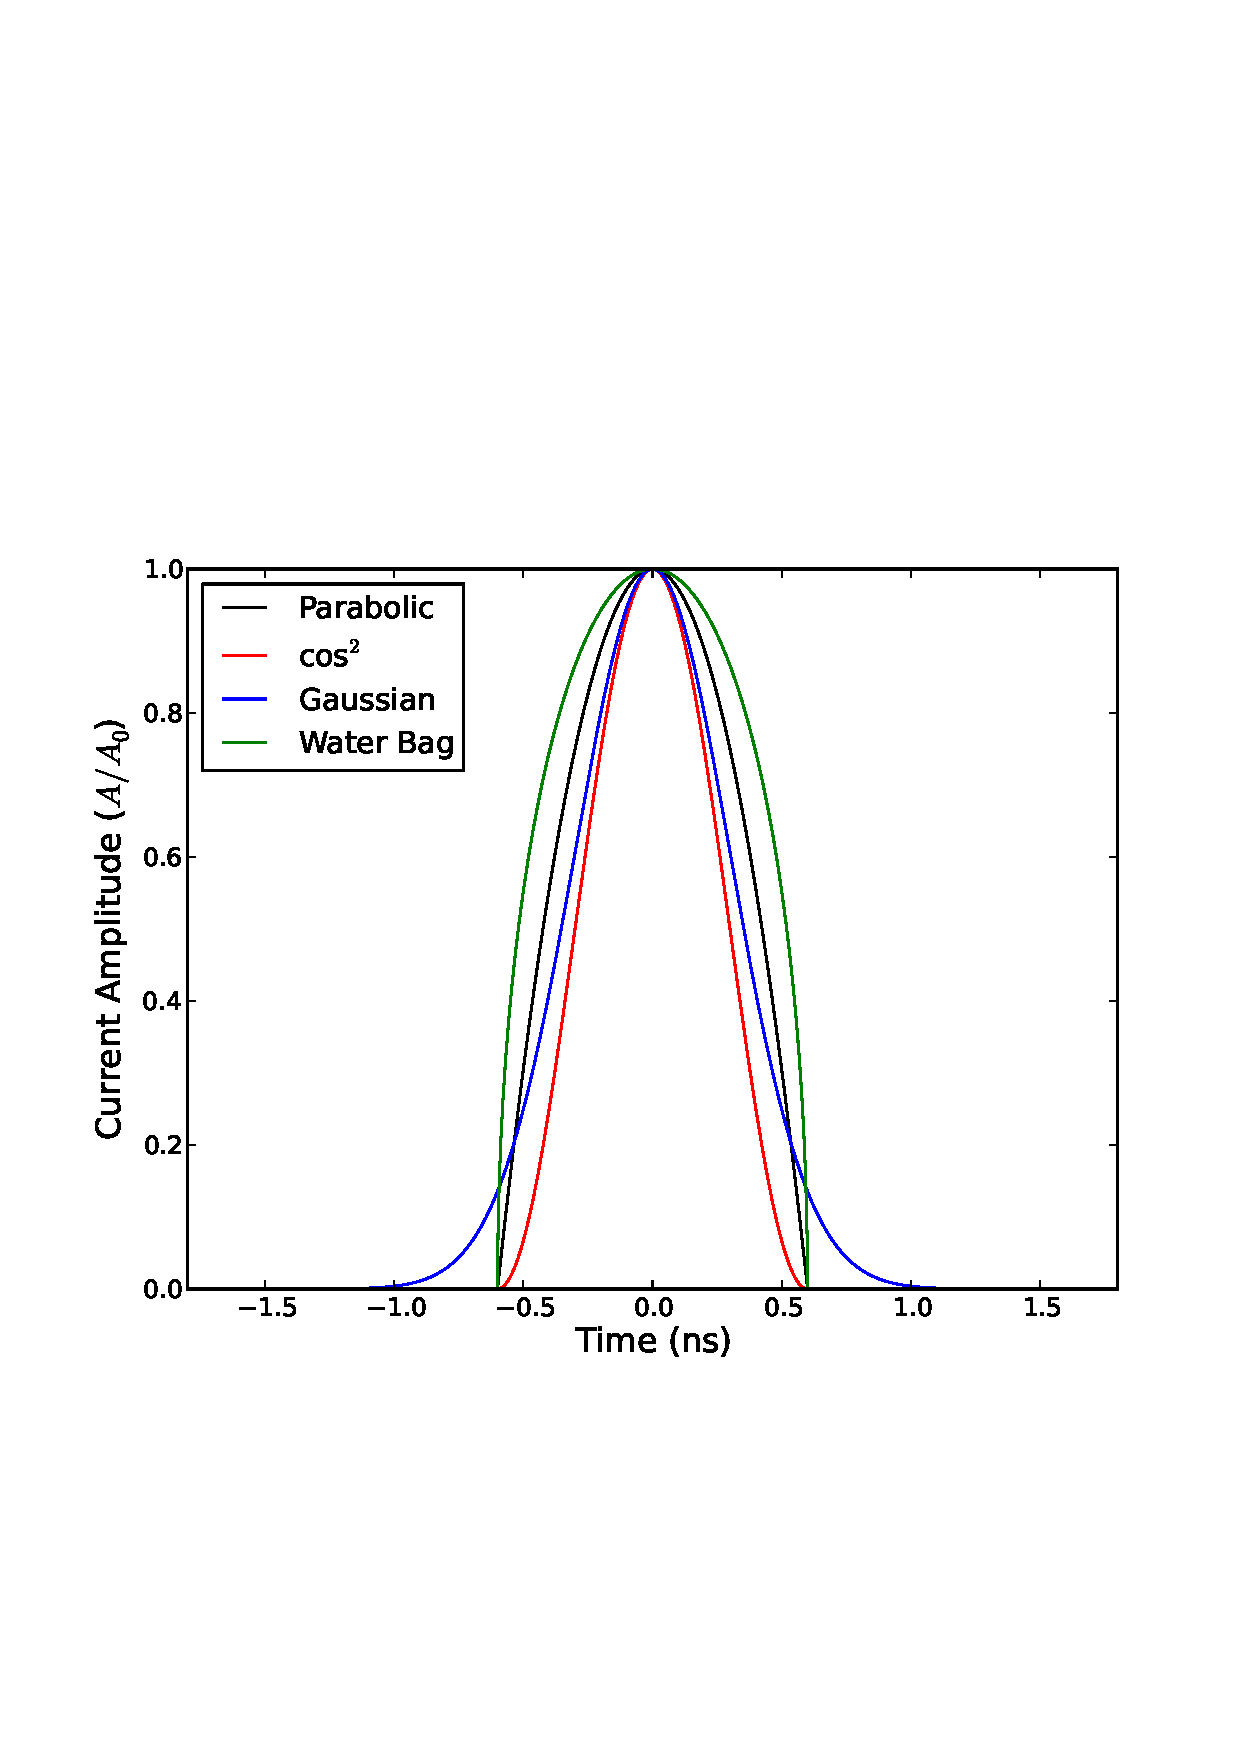
\includegraphics[width=0.65\textwidth]{Wakefields_and_Impedances/figures/bunch_profile_12ns.pdf}
\end{center}
\label{fig:time_bunch_profiles}
\caption{The longitudinal bunch profile of a number of bunch distributions. Note that all of them are normalised to have a peak bunch current of 1. For the gaussian distribution the bunch length is the 4$\sigma$ value. The bunch length $\tau_{b} = 1.2ns$}
\end{figure}

\begin{figure}
\subfigure[]{
\includegraphics[width=0.45\textwidth]{Wakefields_and_Impedances/figures/current_spectrum_12ns.pdf}
\label{fig:current_spec}
}
\subfigure[]{
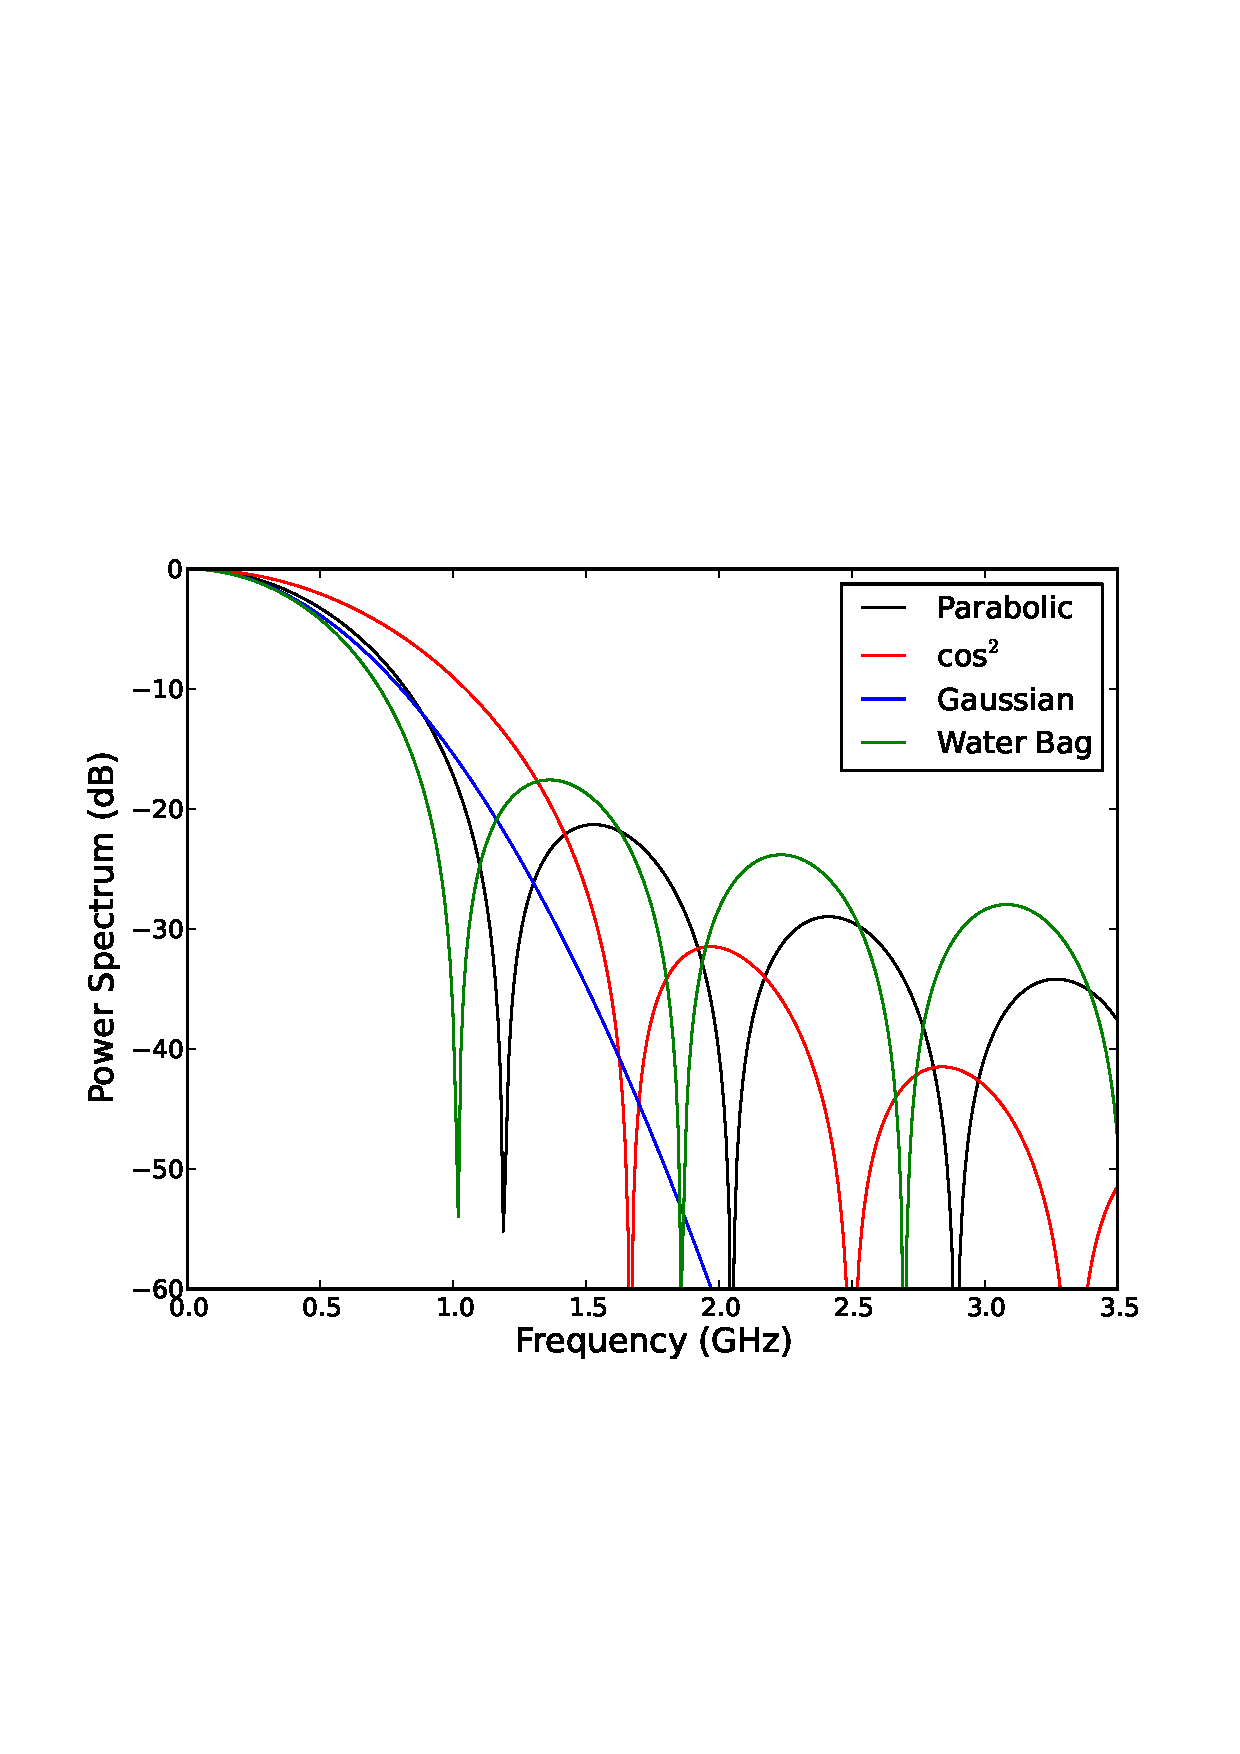
\includegraphics[width=0.45\textwidth]{Wakefields_and_Impedances/figures/power_spectrum_12ns.pdf}
\label{fig:power_spec}
}
\label{fig:freq_dom_prof}
\caption{The frequency domain \ref{fig:current_spec} current spectrum and \ref{fig:power_spec} power spectrum for a number of different bunch profiles with a bunch length $\tau_{b} = 1.2ns$.}
\end{figure}

To illustrate more clearly the effect of changing the bunch length on the power spectrum, a number of bunch profiles and the corresponding power spectra with different bunch lengths are shown below. Firstly, consider a gaussian bunch profile. It can be seen in Fig.~\ref{fig:diff_bunch_len_gauss} that by increasing the bunch length that the magnitude at high frequencies is decreased quite substantially as the bunch length increases. If we consider a finite bunch profile (non-gaussian), we note that we have high frequency lobes. The peak frequency of these lobes depends on the bunch length, as illustrated using a parabolic bunch profile for bunch lengths $\tau_{b} = 1ns, 1.2ns, 1.4ns$ in Fig.~\ref{fig:diff_bunch_len_para}. As the bunch length is increased the lobes move to lower frequencies, and the width of the first branch decreases, as seen for the gaussian bunch. Similar behaviour is observed with the cos$^{2}$ and water-bag bunch profiles.

\begin{figure}
\subfigure[]{
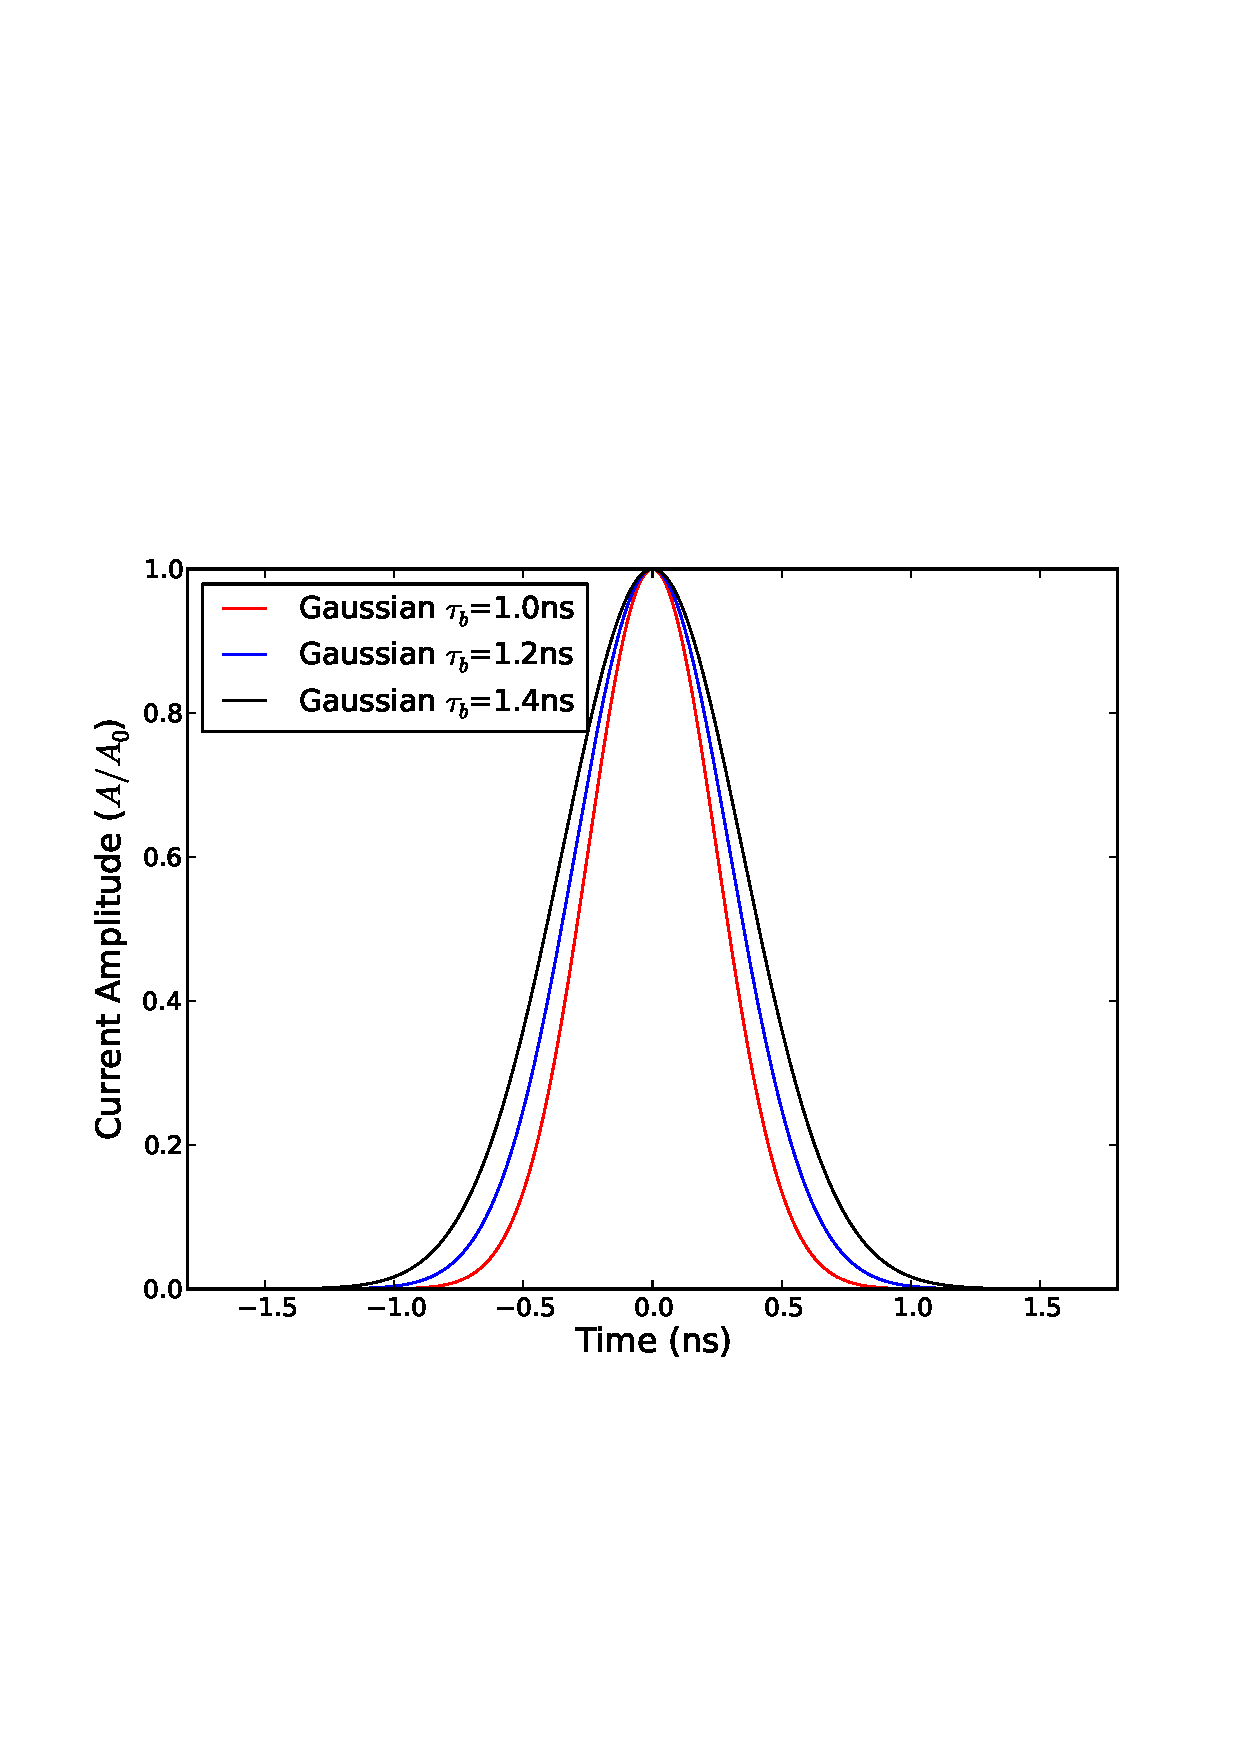
\includegraphics[width=0.45\textwidth]{Wakefields_and_Impedances/figures/gaussian_time_dom_diff_lengths.pdf}
\label{fig:change_len_time_gauss}
}
\subfigure[]{
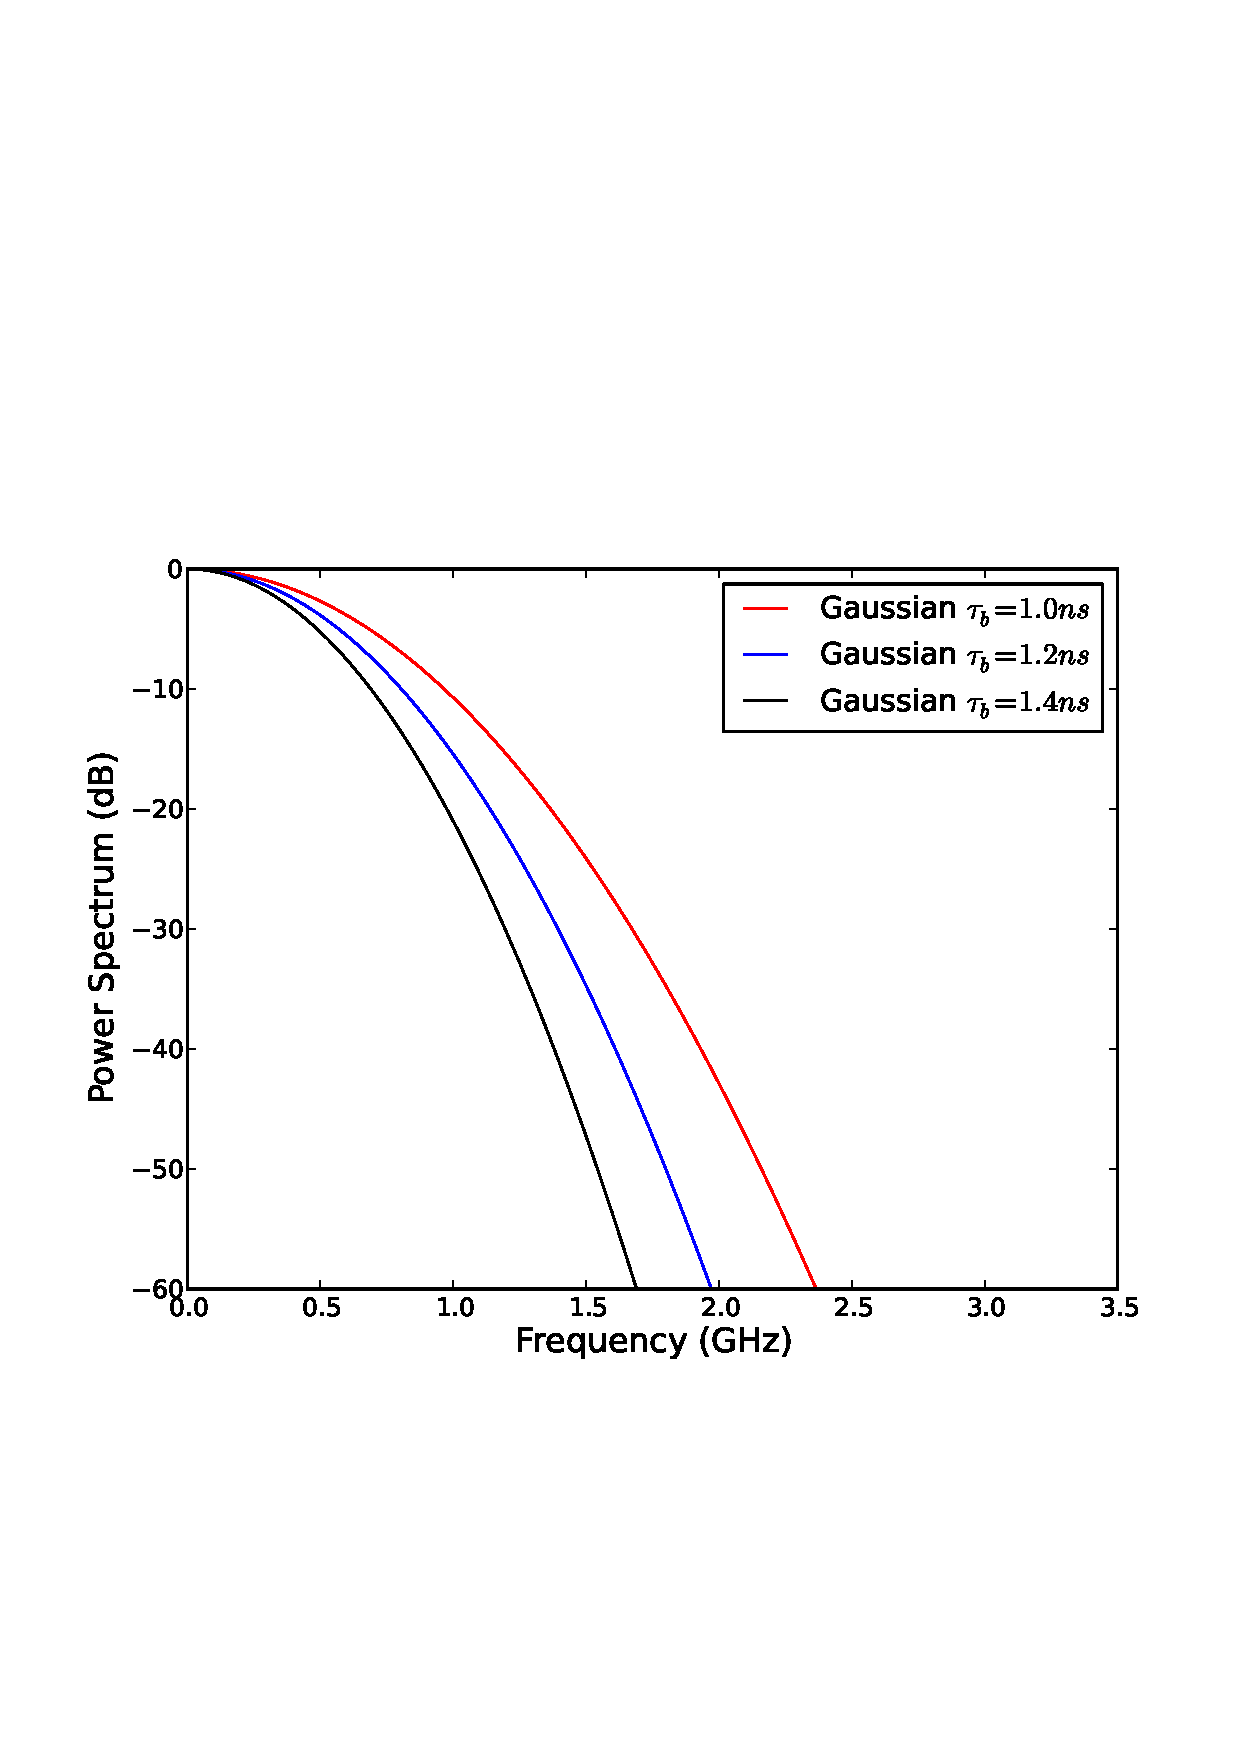
\includegraphics[width=0.45\textwidth]{Wakefields_and_Impedances/figures/gaussian_power_spec_diff_lengths.pdf}
\label{fig:change_len_freq_gauss}
}
\caption{\ref{fig:change_len_time_gauss} The longitudinal profile and the \ref{fig:change_len_freq_gauss} associated bunch power spectrum for a number of bunch lengths assuming a gaussian bunch profile.}
\label{fig:diff_bunch_len_gauss}
\end{figure}

\begin{figure}
\subfigure[]{
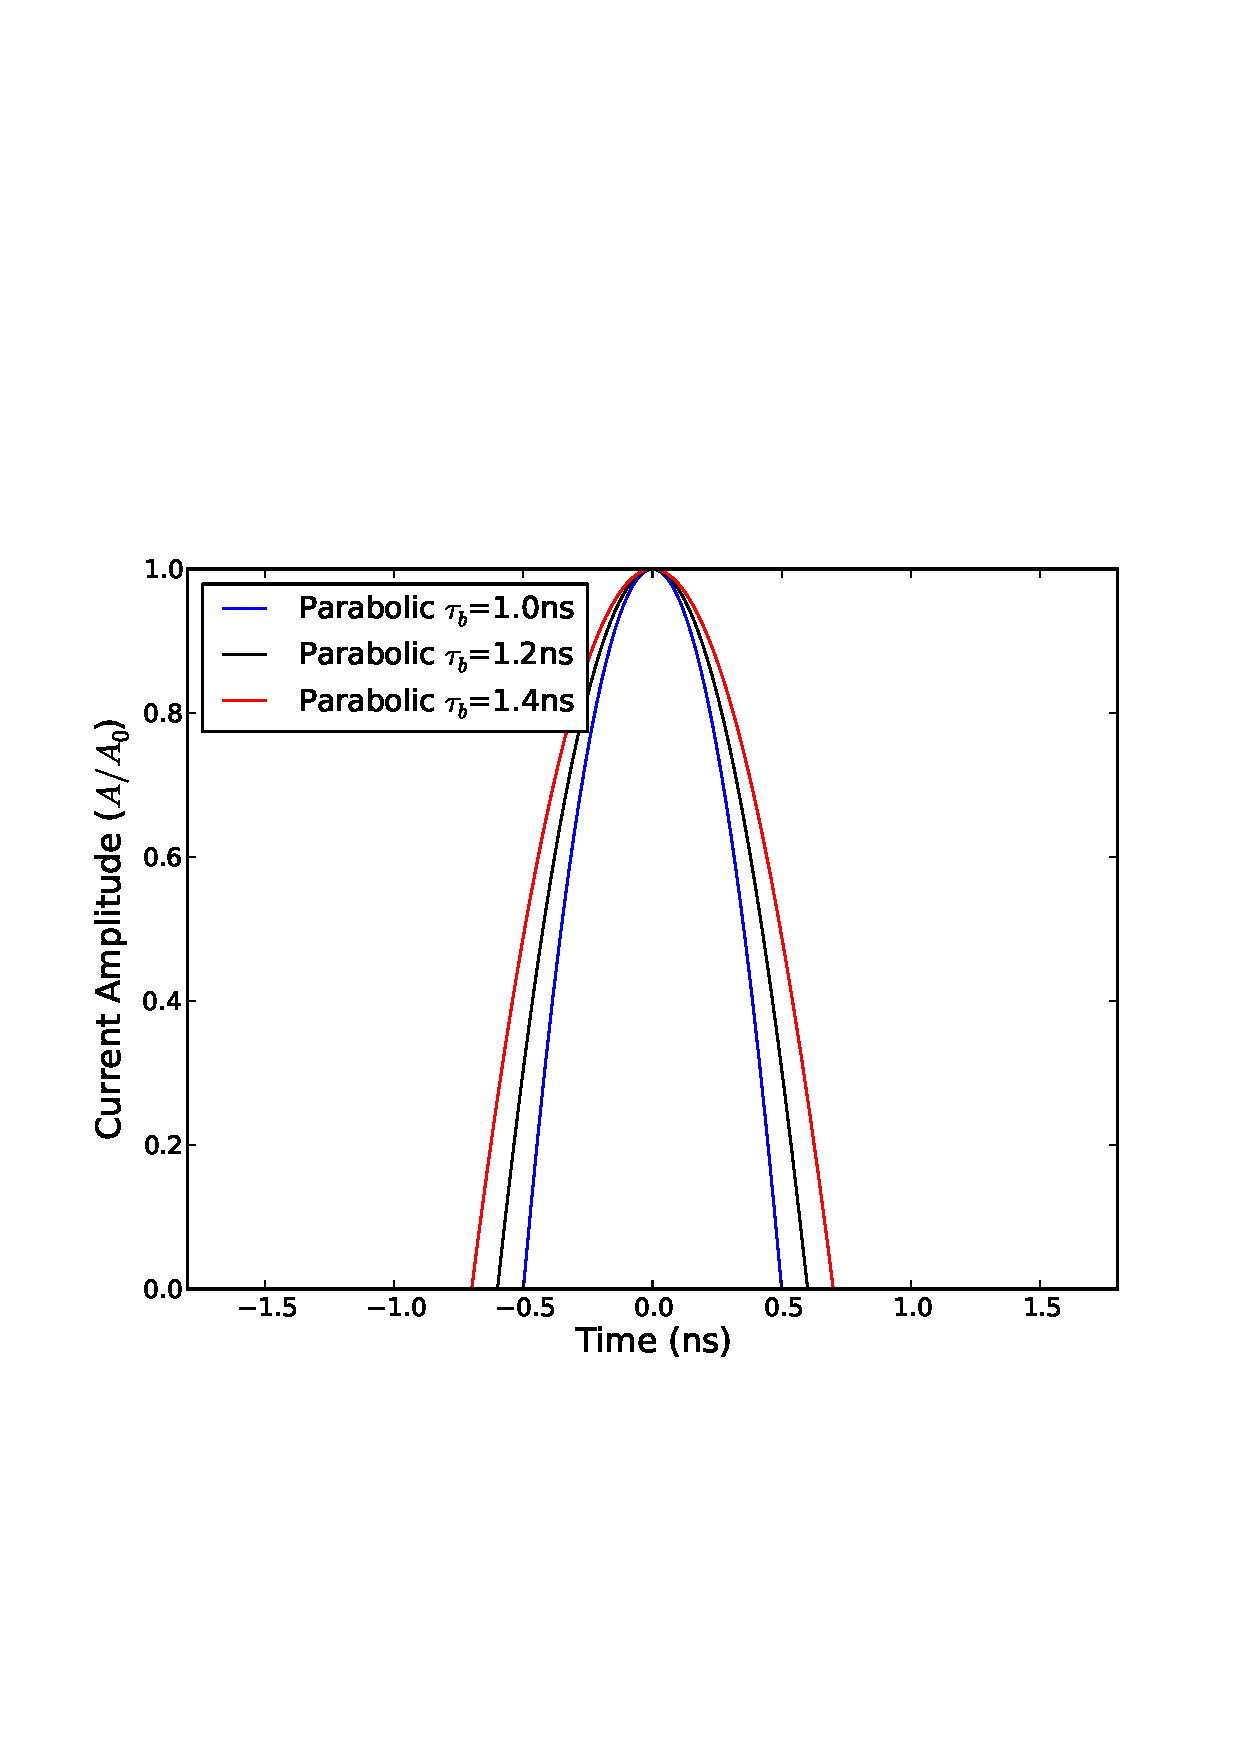
\includegraphics[width=0.45\textwidth]{Wakefields_and_Impedances/figures/current_amp_para_change.pdf}
\label{fig:change_len_time_para}
}
\subfigure[]{
\includegraphics[width=0.45\textwidth]{Wakefields_and_Impedances/figures/freq_power_para_change.pdf}
\label{fig:change_len_freq_para}
}
\caption{\ref{fig:change_len_time_para} The longitudinal profile and the \ref{fig:change_len_freq_para} associated bunch power spectrum for a number of bunch lengths assuming a parabolic bunch profile.}
\label{fig:diff_bunch_len_para}
\end{figure}

Finally, a comparison of a measured bunch power spectra and the analytical power spectra is shown in Fig.~\ref{fig:power_all}. It can be seen that whilst it is possible to replicate some of the properties of the measured spectrum, an exact replication is non-trivial. Further investigation into the appropriate bunch profile is ongoing.

\begin{figure}
\begin{center}
\includegraphics[width=0.65\textwidth]{Wakefields_and_Impedances/figures/beam_spectra_power_12ns.pdf}
\end{center}
\label{fig:power_all}
\caption{A comparison of a measured beam power spectrum and a number of analytical bunch profiles assuming a bunch length of 1.2ns.}
\end{figure}



% Introduce a number of longitudinal profiles in time domain - gaussian, parabolic line density, cos^2, water bag - comments of realism (gaussian being infinite) - truncated gaussian
% Comparison in the frequency domain - firstly gaussian compared to truncated gaussian - infinite tails reduce the magnitude of the higher frequency components and lobe
% Gaussian, parabolic, cos^2 - all with the same bunch length
% Using the above examples try using a number of different bunch lengths to illustrate how they change (gaussian - just extends further, parabolic, cos^2 lobe frequency changes)
% Finally - comparison to measured spectra to illustrate changes in bunch length and frequency components as bunch is ramped and squeezed

\section{Beam induced heating due to a low Q impedance}

For an impedance with a characteristic Q that is small (Q $<$ 10), it can be seen that the impedance peak will interact substantially with a number of beam harmonics (see Fig.~\ref{fig:low_q_harmonics}) due to the broad frequency range it occupies.

\begin{figure}
\begin{center}
\includegraphics[width=0.65\textwidth]{Wakefields_and_Impedances/figures/low_q_10_resonance_beam_harmonics.pdf}
\end{center}
\label{fig:low_q_harmonics}
\caption{The beam harmonics of a beam with a bunch spacing of 25ns overlayed on the real component of the longitudinal impedance an example of a low Q impedance ($R_{s}=10\omega$, Q = 10, $f_{res}=1GHz$). The blue lines represent the frequency of a beam harmonic, not necessarily the magnitude of the power spectrum at that point. Note that a number of beam harmonics overlay non-zero impedance values.}
\end{figure}

Further investigation of the longitudinal beam spectrum reveals that there is significant structure between the major harmonics (which are due to the bunch spacing of the beam) which can be attributed to the other time structures of the beam, for example the bunch train spacing, or the interval between the pilot bunch train and the subsequent bunch train. As such the treatment of the estimation of beam losses requires a broad spectrum approach. If we consider Eqn.\ref{eqn:power_loss_omega} we see that we can treat the power losses in an integral form. We can observe a number of properties using this assumption. The power loss is proportional to the beam properties in the following manner:

\begin{enumerate}
\item{$P_{loss} \propto N^{2}$}
\item{$P_{loss} \propto n_{bunch}$}
\end{enumerate}

\section{Beam induced heating due to a high Q impedance}

In contrast to the overlap of the beam spectrum with a low Q impedance, for a high Q impedance only one beam harmonic lies upon the resulting impedance to any significant quantity. This is illustrated in Fig~\ref{fig:high_q_harmonics} If we consider Eqn \ref{eqn:heating-gen} and consider the situation where

\begin{equation}
\left( 2 \left| \lambda \left(p \omega_{rev}n_{bunch} \right)  \right|^{2}  \Re{}e \left( Z_{\parallel} \left(p \omega_{rev}n_{bunch}\right) \right) \right) = 
\begin{cases}
\left( 2 \left| \lambda \left( \omega_{res} \right)  \right|^{2}  \Re{}e \left( Z_{\parallel} \left( \omega_{res} \right) \right) \right) &\textrm{if $p \omega_{rev} n_{bunch} = \omega_{res}$}\\
0								&\textrm{if $p \omega_{rev} n_{bunch} != \omega_{res}$}
\end{cases}
\label{eqn:single_harmonic_profile}.
\end{equation}

\begin{figure}
\begin{center}
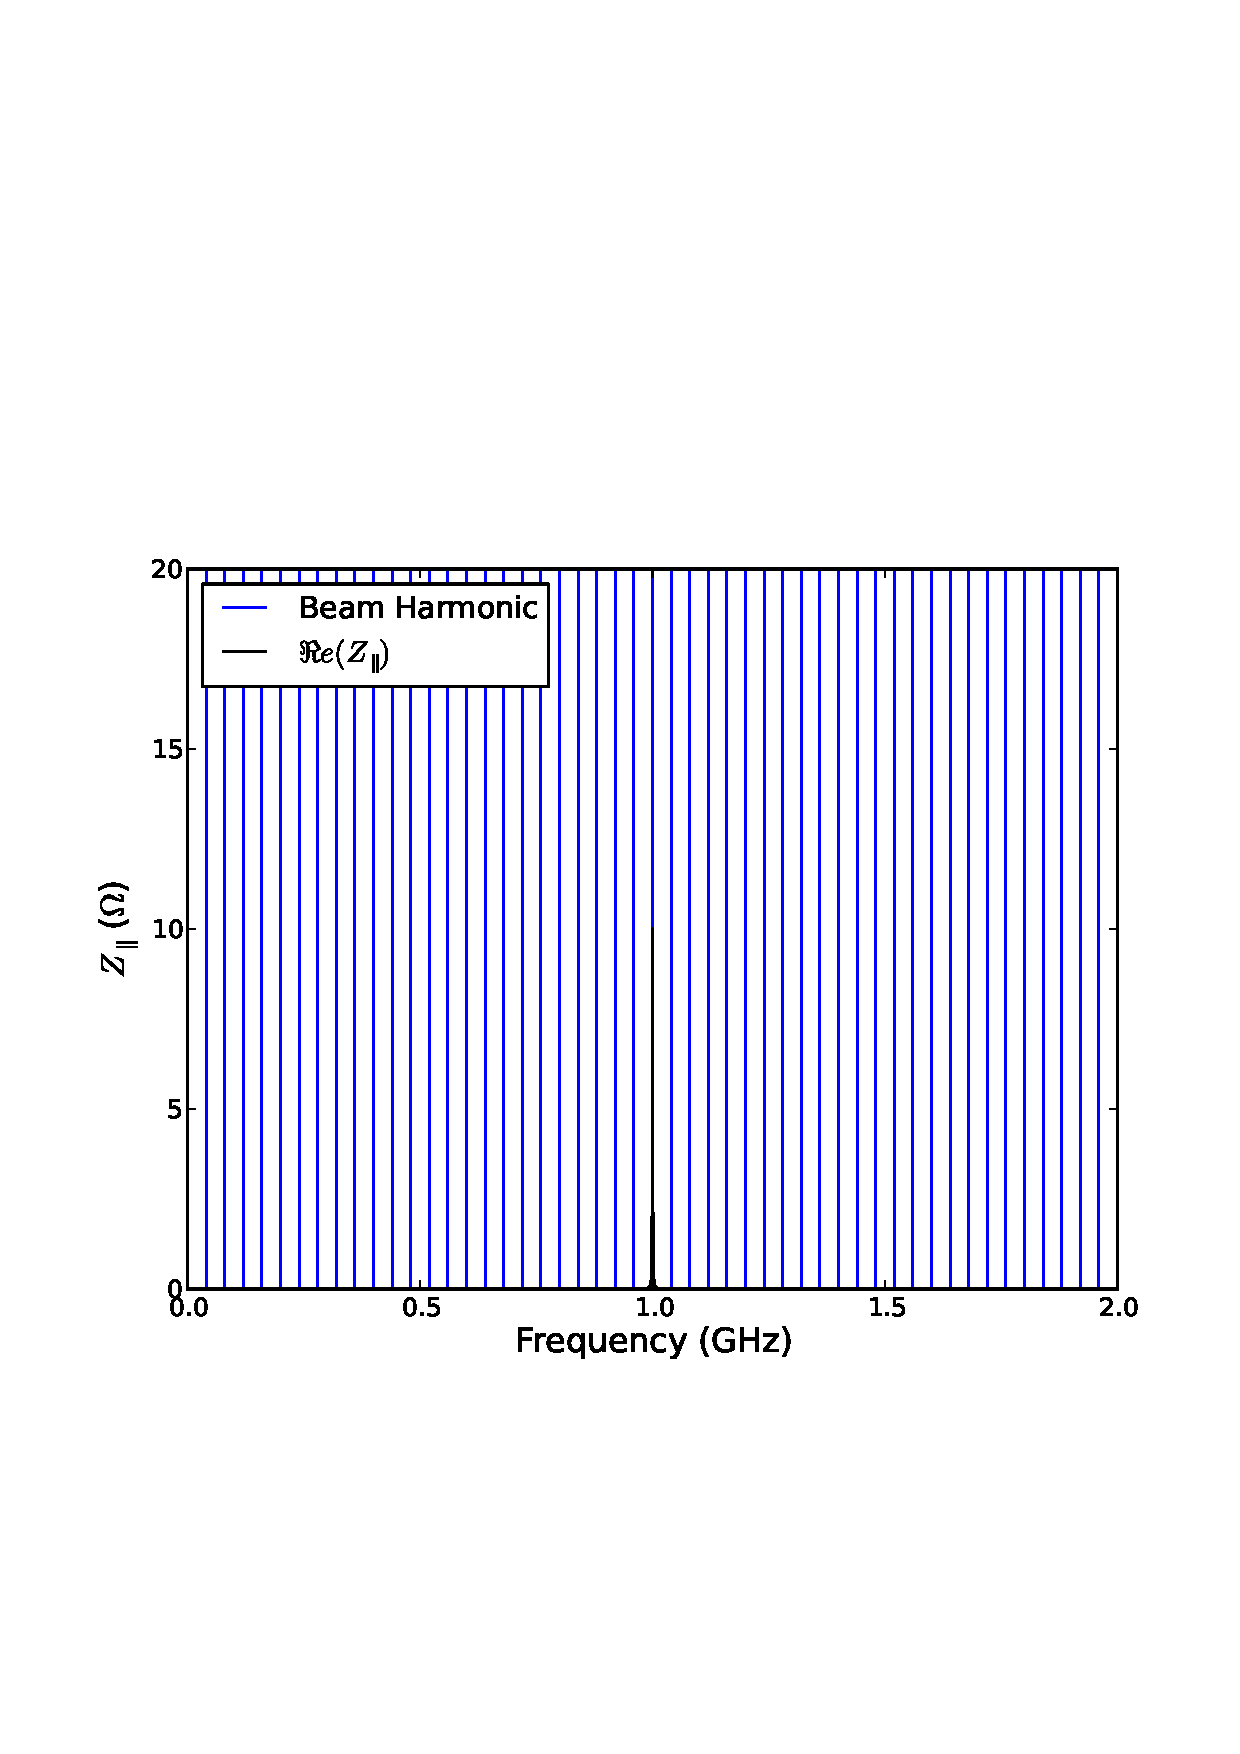
\includegraphics[width=0.65\textwidth]{Wakefields_and_Impedances/figures/high_q_1000_resonance_beam_harmonics.pdf}
\end{center}
\label{fig:high_q_harmonics}
\caption{The beam harmonics of a beam with a bunch spacing of 25ns overlayed on the real component of the longitudinal impedance an example of a high Q impedance ($R_{s}=10\omega$, Q = 1000, $f_{res}=1GHz$). The blue lines represent the frequency of a beam harmonic, not necessarily the magnitude of the power spectrum at that point. Note that only a single beam harmonic overlays a non-zero impedance values.}
\end{figure}

It can then be seen that Eqn~\ref{eqn:heating-gen} simplifies to

\begin{equation}
P_{loss} = \left( \omega_{rev}eN_{b}n_{bunch}  \right)^{2}  \left( 2 \left| \lambda \left( \omega_{res} \right)  \right|^{2}  \Re{}e \left( Z_{\parallel} \left(\omega_{res} \right) \right) \right). 
\label{ean:heating-high-q}
\end{equation}

The following properties can subsequently be seen as a result:

\begin{enumerate}
\item{$P_{loss} \propto N^{2}$}
\item{$P_{loss} \propto n_{bunch}^{2}$, provided that the resonant frequency of the resonance continues to coincide with a beam harmonic.}
\end{enumerate}

\section{Some Examples of the Beam-Induced Heating}

In this section we shall illustrate some important factors that have been covered in previous sections. In particular, the interaction of different bunch profiles at different bunch lengths with an example cavity resonance will be covered in some detail to illustrate how the estimated heating can change drastically depending on higher frequency lobes in the beam current spectrum. In addition, the heating due to two particle beams in the same vacuum chamber shall be briefly covered for interest.

\subsection{The Effect of Bunch Length on Power Loss}

As can be seen in Figs.~\ref{fig:freq_dom_prof} and \label{fig:diff_bunch_len_para}, the bunch profile and the bunch length can significantly alter the magnitude of the beam current at higher frequencies. To illustrate this, let us consider two resonant impedances, one broadband $Z_{bb}$ and one narrow band $Z_{nb}$ impedance, characterised by having a low-$Q$ and a high-$Q$ respectively. Both impedances shall have the same resonant shunt impedance $R_{s} = 100\Omega$. The broadband impedance shall have a $Q_{bb}=1$, and the narrow band impedance $Q_{nb}=1000$. The resonant frequency will be changed to illustrate effects in different regimes of the bunch length and of different bunch profiles.

We shall use the gaussian bunch profile and the $cos^{2}$ bunch profile for these examples. The gaussian is useful to illustrate the effect of just the changing bunch length, and the $cos^{2}$ due to the presence of a high frequency lobe in it's frequency domain current spectrum. The $cos^{2}$ frequency domain current profile is given by

\begin{equation}
I \left( \omega \right) = \frac{sin \left( \omega \tau_{b}/2 \right)}{ \omega \tau_{b}/2 \left[ 1 - \left(  \omega \tau_{b}/2 \right)^{2}  \right]}.
\end{equation}

First we shall consider a narrowband impedance which has a resonant frequency $\omega_{0} =2GHz$ which falls upon a beam harmonic such that $\omega_{0}=n\omega_{rev}$ where n is an integer. It should be noted that for other cases the contribution of these sources of heating is negligible due to the small beam current at this frequency. There are two extreme cases; that of  $\omega_{0} \gg 1/\tau_{b}$, in which it can be seen that the current spectrum will be negligible at the frequency of the impedance, and $\omega_{0} \ll 1/\tau_{b}$ where the beam current spectrum is essentially the same as the DC spectral component. The transition in this intervening regime is shown in Fig~\ref{fig:bunch_length_heat_narrow}, assuming a bunch current of 1A. It can be seen that in this case the heating falls drastically as the bunch length increases.

\begin{figure}
\begin{center}
\includegraphics[width=0.8\textwidth]{Wakefields_and_Impedances/figures/heating_narrowband_gauss_bunch_length.pdf}
\end{center}
\label{fig:bunch_length_heat_narrow}
\caption{The change in power loss due to a narrow band resonance characterised by $\omega_{0} = 2GHz$, $R_{s} = 100\Omega$, $Q = 1000$ with a gaussian bunch distrbution of different lengths.}
\end{figure}

If we instead consider a cos$^{2}$ distribution we instead see the effect of the secondary lobes in the beam current spectrum. The power loss with bunch length is shown in Fig.~\ref{fig:bunch_length_heat_narrow_cos} in comparison to that of the gaussian profile. The beam power spectrum for a number of different bunch lengths are shown with the real component of the longitudinal impedance in Fig.~\ref{fig:imp_profile_cos}. Here it can be clearly seen that the intersection of the secondary lobe with the resonant impedance causes a peak in the power lost by the beam, highlighting the neccessity to be aware of the resonant frequencies of resonant impedances with relation to the beam harmonics.


\begin{figure}
\subfigure[]{
\includegraphics[width=0.5\textwidth]{Wakefields_and_Impedances/figures/heating_narrowband_gausscos_bunch_length.pdf}
\label{fig:long_imp_narrow_current}
}
\subfigure[]{
\includegraphics[width=0.5\textwidth]{Wakefields_and_Impedances/figures/impedance_and_power_cos_res.pdf}
\label{fig:imp_profile_cos}
}
\caption{\ref{fig:long_imp_narrow_current} The change in power loss due to a narrow band resonance characterised by $\omega_{0} = 2GHz$, $R_{s} = 100\Omega$, $Q = 1000$ interacting with a cos$^{2}$ bunch distribution with different bunch lengths. The impedance and the beam power spectrum are shown in \ref{fig:imp_profile_cos} to illustrate how this relates to the power loss.}
\end{figure}

For the broadband heating we shall consider a resonant impedance defined by the following parameters, $\omega_{0} = 2GHz$, $Q=1$, $R_{s}=100\Omega$. To account for the multiple beam harmonics that will interact with the resonance, it is assumed that the beam harmonics in this case occur at $20$MHz intervals. The impedance and the beam power spectrum is shown in Fig.~\ref{fig:broadband_heat_bunch_len} and the resulting power loss in Fig.~\ref{fig:broadband_power_loss} where it can be seen that the power loss decreases slowly with increasing bunch length. This is due to the significant contribution to the power loss at low frequencies, in which the component of the beam power spectrum decreases only marginally due to the decreasing bunch length.

\begin{figure}
\subfigure[]{
\includegraphics[width=0.5\textwidth]{Wakefields_and_Impedances/figures/heating_broadband_gausscos_bunch_length.pdf}
\label{fig:broadband_heat_bunch_len}
}
\subfigure[]{
\includegraphics[width=0.5\textwidth]{Wakefields_and_Impedances/figures/impedance_and_power_cos_res_broad.pdf}
\label{fig:broadband_power_loss}
}
\caption{\ref{fig:broadband_heat_bunch_len} The change in power loss due to a narrow band resonance characterised by $\omega_{0} = 2GHz$, $R_{s} = 100\Omega$, $Q = 1$ interacting with a cos$^{2}$ bunch distribution with different bunch lengths. The impedance and the beam power spectrum are shown in \ref{fig:broadband_power_loss} to illustrate how this relates to the power loss.}
\end{figure}

\subsection{Beam-Induced Heating due to two traversing beams}

Previous work [cite A. Grudiev TCTVB/TCLIA] has investigated the effect of two beams in a vacuum on the beam-induced heating. This is restated here for the sake of completeness.

To begin, consider the two currents $I_{b1} = I_{0}e^{i\phi_{1}}$ and $I_{b1} = -I_{0}e^{i\phi_{2}}$ representing two counter rotating beams. $I_{0}$ represents the beam current, and $\phi_{1/2}$ the phase of beam 1 and beam 2 respectively. Each beam also sees a seperate potential when it traverses the impedance, given by $V_{b1} = \int_{b1} E_{z} e^{i\omega_{0}z/c} dz$ and $V_{b2} = \int_{b2} E_{z} e^{i\omega_{0}z/c} dz$ respectively. By Ohms law it can then be seen that

\begin{equation}
\begin{pmatrix}
V_{b1} \\
V_{b2}
\end{pmatrix}
=
\begin{bmatrix}
Z_{11} & Z_{12} \\
Z_{21} & Z_{22}
\end{bmatrix}
\begin{pmatrix}
I_{b1} \\
I_{b2}
\end{pmatrix}.
\end{equation}

The power loss due to both beams can then be seen to be

\begin{equation}
P_{loss} = \begin{pmatrix}
V_{b1} & V_{b2}
\end{pmatrix}
\begin{pmatrix}
I_{b1} \\
I_{b2}
\end{pmatrix}^{*}.
\end{equation}

In the worst case scenario, the values of the impedance matrix are real, and are equal in value to the peak values of the resonant impedance
\begin{equation}
Z_{11} = 2R^{b1}_{s};\text{    } Z_{22} = 2R^{b2}_{s};\text{    }  Z_{12} = Z_{21} = 2 \sqrt{R^{b1}_{s}R^{b2}_{s}}.
\end{equation}

The power loss then becomes

\begin{equation}
P_{loss} = I_{0}^{2} 2 \left( R_{s}^{b1} +  R_{s}^{b1} - 2\sqrt{R^{b1}_{s}R^{b2}_{s}} cos \left( \delta \phi \right) \right)
\end{equation}

where $\delta \phi = \phi_{1} - \phi_{2}$ is the phase difference between beam 1 and beam 2. This can be found relatively easy by comparing the distance $\delta s$ from a collision IP of the machine. Assuming the beams are ultrarelativistic $\delta \phi = \omega_{rev} 2  \delta s /c$. It can then be seen that the the last term may either reduce or increase the power loss depending on whether $cos\left( \delta \phi \right) = 1$ or $cos\left( \delta \phi \right) = -1$ respectively.



\subsection{Single Bunch and Coupled Bunch Instabilities}

\begin{itemize}
\item{Take references to introductory section on beam dynamics - longitudinal and transverse oscillations}
\item{Introduce bunch oscillation spectra - resonance diagrams for transverse motion, longitudinal spectra}
\item{Instabilities by resonance crossing, LMCI, TMCI, headtail instabilities, TCBI}
\item{Section on landau damping/transverse dampers? Other way to counter large impedances.}
\end{itemize}

\subsection{Example of LMCI with Broadband and Space Charge Impedances Studied with HEADTAIL}

%
% Theory of LMCI (potential well distortion and microwave instability)
% Simulations with BB, SC and BB/SC impedances
% Comparison of different impedances and their production of different stability criteria
%

\chapter{Bench Top Measurements of Beam Coupling Impedance}
%

Due to the sensitivity of the beam coupling impedance to the boundary conditions of the equipment used, it is necessary to utilise different measurement techniques to fully analyse the impedance of accelerator structures.

\section{Low Q-factor Impedances}

For structures that are expected to contain mostly low Q-resonances (i.e. resistive wall impedance) it is appropriate to use the coaxial wire method[ref], sometimes also called the stretched wire method. This method relies on the similarity of the electromagetic field profile due to an ultrarelativistic charged particle and that of a short electrical pulse sent along a coaxial wire. 

An moving charged particle produces an electromagnetic field in a arc transverse to its direction of motion, where the angle of the arc opening is proportinal to the relativistic factor of the particle $\gamma$. For an ultrarelativistic particle ($\gamma \leftarrow \infty$), the field becomes entirely perpendicular to the direction of motion. If we place a conductive wire along the same path we would expect the charged particle to take (in most cases this is well represented by a straight wire), a short electrical pulse sent along this wire would propogate in the TEM (transverse electrical and magnetic field) mode, producing a field profile similar to that emitted by the ultrarelativistic charged particle (see. Fig. \ref{fig:coax-part-profile})


\begin{figure}

\caption{Comparison of the electromagnetic field profile of a moving charged particle and a short time pulse propogating along a coaxial wire.}
\label{fig:coax-part-profile}
\end{figure}

\subsection{Classical Coaxial Wire Method}

The classical coaxial wire method, first proposed by V. Vaccarro in 1990 [ref], is a transmission method that measures the complex transmission coefficient of a DUT (Device Under Test) made up of the equipment whose impedance is to be measured and a coaxial wire passing through it. 

The experimental setup is as shown in Fig. \ref{fig:classic-coax}. Firstly the external circuit (i.e. everything not the DUT) is matched to the characteristic impedance of the coaxial line inside the DUT. This is done by measuring the reflection coefficient $\Gamma$ for the setup with only one port connected to the DUT and the other end terminated by an open connection. Knowing the characteristic impedance of the VNA and associated cables (typically $Z_{0} = 50\Omega$), we can easily calculate the characteristic impedance, $Z_{c}$, from the relation,

\begin{equation}
\Gamma = \frac{Z_{c} - Z_{0}}{Z_{c} + Z_{0}}.
\end{equation}

We then electrically match the characteristic impedance by adding resistors in series just before the DUT to resistively match the characteristic impedance of the VNA to that of the DUT. It is possible to use physical matching also using transition cones but these are costly, time consuming to construct and require new cones for each piecof equipment measured. And as can be seen in Fig. \ref{fig:matching-plot}, matching with a resistor is highly effective at removing the presence of reflections in coaxial measurements.

\begin{figure}

\caption{Experimental setup for a measurement of the beam coupling impedance using the classical coaxial wire method}
\label{fig:classic-coax}
\end{figure} 

\begin{figure}

\caption{An example of a reflection measurement made with and without a matching resistor. The faded line is the measurement without matching, the bold line that with. The reduction in the reflection can be seen.}
\label{fig:matching-plot}
\end{figure}

The value that we wish to measure to evaluate the beam coupling impedance of a device are the scattering parameters of the resulting circuit, in particular $S_{21}$, the normalised transmission parameter through the DUT. $S_{21}$ is calculated by taking the measured transmission parameter $S_{21,DUT}$ and dividing it by the transmission parameter through a reference line of the same physical length as the DUT,

\begin{equation}
S_{21} = \frac{S_{21,DUT}}{S_{21,REF}}
\end{equation}.

The effect of this is to correct the measured phase change in the DUT to be that only caused by the imaginary component of the beam coupling impedance.

There are subsequently a number of ways to evaluate the beam coupling impedance of the DUT depending on it's expected properties. For devices that are expected to have a either a small impedance, or those that are physically very short in length, it is possible to use the so called lumped impedance formula[ref];

\begin{equation}
Z = 2Z_{c} \frac{1-S_{21}}{S_{21}}
\end{equation}.

For distributed impedances, it is suitable to use the so called log formula (called so due to attenuation causing a log function to appear in the evaluation),

\begin{equation}
Z = -2Z_{c} ln \left( S_{21} \right)
\end{equation}.

For long components or measurements at very high frequencies there exists the improved log formula. This takes into account more completely the electrical length of the device, given by

\begin{equation}
Z = -2Z_{c} ln \left( S_{21}  \right) \left( 1 + j\frac{ln \left( S_{21}\right) }{2\Theta}  \right)
\end{equation}

where $\Theta = 2\pi \frac{L}{\lambda}$ is the normalised electrical length of the device, $L$ the length of the device, $\lambda$ the wavelength of the frequency of measurement. It is possible to see that the lumped impedance formula can be used when $\Theta \leq 1$, and the improved log formula becomes useful for $\Theta \geq 5$[erk's paper].




\subsection{Resonator Coaxial Wire Method}

An alternative method for measuring the beam coupling impedance is by using the so called resonator method. The setup for this method is similar to that of the classical coaxial wire method, except that the matching resistor network between the VNA and DUT is replaced by a weak capacitive coupling ($S_{11} < 0.5dB$) at both ends of the DUT. This then produces a structure which resonates at frequencies where the wavelength corresponds to the classical closed structure form,

\begin{equation}
\lambda = \frac{2L}{n}
\end{equation}

where $\lambda$ is the wavelength of the resonance, n the harmonic of the resonance and L the length of the device. 

The resonant method enables accurate measurement of the transmission losses due to the real longitudinal impedance. Additional advantages are that no matching is required, and a large number of mechanical uncertainties (electrical connections, consistency of calibration) can be avoided. However it can be seen that the frequency resolution is limited due to the length of the DUT so the method is not recommended as the only measurement method for structures expected to contain high-Q, narrowband resonances. It can however be used to corroborate the results obtained using the classical method.

For each resonancce peak, the loaded Q-factor and the frequency of the resonance are measured. For a weak coupling at both ends of the DUT, we can write the coupling coefficient k as

\begin{equation}
k = \frac{\left| S_{21} \right|}{1 - \left| S_{21} \right| }.
\label{eqn:coupling_coeff}
\end{equation}

The difference between the unloaded $Q$-factor, $Q_{0}$ , and the loaded $Q$-factor, $Q_{L}$, is a function of k. We can get an approximate correction by using the formula

\begin{equation}
Q_{0} = Q_{L} \left( 1 + k  \right).
\label{eqn:Q_correc}
\end{equation}

Subsequently the measured line attenuation (in Np/m) is then calculated

\begin{equation}
\alpha_{m} = \frac{\pi}{\lambda Q_{0}}.
\label{eqn:atten}
\end{equation}

Note that this attenuation includes both that from the beam coupling impedance due to the finite resistance of the wire material. We can estimate the attenuation due to the wire material as

\begin{equation}
\alpha_{w} = \sqrt{\pi \rho_{w} \epsilon f} \frac{1}{d ln D/d}
\label{eqn:wire_atten}
\end{equation}

where $\rho_{w}$ is the wire resistivity, $\epsilon$ the permitivitty, $f$ the frequency, $d$ the diameter of the inner conductor and $D$ the diameter of the outer conductor. At very low frequencies the finite skin depth of the inner conductor would also have to be taken into account. Using the corrected attentuation $\alpha = \alpha_{m} - \alpha_{w}$, the real longitudinal impedance per unit length can be found to be 

\begin{equation}
\Re e\left\{ Z \right\} = 2Z_{c} \alpha
\label{eqn:res_imp}
\end{equation}

\begin{figure}

\label{fig:res-resonancce-examples}
\caption{An example of the resonance pattern seen whilst performing measurements using the resonant method. Each peak corresponds to one data point in the final measurements.}
\end{figure}

To calculate the imaginary impedance using the resonant method involves a more involved calculation. In particular it is necessary to carry out measurements using the resonant method on a reference pipe of the same physical length to the DUT, either using physical measurements or a simulated measurement.

If we consider the complex impedance of the two measurements, $Z_{DUT}$ for the DUT and $Z_{REF}$ for a perfectly conducting reference pipe, we can simplify them as

\begin{align}
Z_{DUT} & =  R + jX_{1}  =  Z_{1}e^{j \phi} \\
Z_{REF} & =  jX_{2}  =  Z_{2}e^{j.0}
\end{align}

where $R$ is the resistive component of the DUT impedance, $X_{1/2}$ the imaginary component of the impedance (DUT and reference pipe respectively), $\phi$ is the angle of DUT impedance projected onto a complex plane and $Z_{2} = \sqrt{R^{2} + X^{2}}$. If we consider a measured value depedent on the impedance, for example the transmission parameter $S_{21}$ at a resonance peak, we have the following relations

\begin{align}
S_{21}^{DUT} = S_{0}e^{j \left( \omega_{1}t + \phi \right)} \\
S_{21}^{REF} = S_{0}e^{k \left( \omega_{2}t \right)}
\end{align}

where $S_{0}$ is some normalised scalar, $\omega_{1/2}$ is the frequency of the resonance and $t = \frac{L}{c}$ . Thus for a pair of corresponding peaks from resonance measurements for which we have measured $\omega_{1}$ and $\omega_{2}$ we can equate $S_{21}^{DUT} = S_{21}^{REF}$ and thus show

\begin{equation}
\phi = t \left( \omega_{2} - \omega_{1} \right).
\end{equation}

Subsequently we can see that

\begin{equation}
X = Z_{DUT} sin \phi = R \frac {sin \phi}{cos \phi} = R tan \phi
\end{equation}

where $R = \Re e(Z)$.

\subsection{Transverse Impedance Measurements}

The above methods give a general impression of how to carry out coaxial wire measurements of the impedance of accelerator components. Directly applied as described they allow the measurement of the longitudinal impedance of a DUT. However, from a beam stability point of view it is often more interesting to look at the transverse imedance of a device. In particular it would be useful to have a method of determining the vertical/horizontal dipolar (or driving) impedance and the vertical/horizontal quadrupolar (detuning) impedance of any device. In this section we describe how do this for structures with top/bottom, left/right symmetry and then generalising to asymmetric structures, with illustration from simple examples evaluated using simulations.

To allow a complete explanation of how to verify the methods of measuring transverse impedances, let us first consider the general form of the $m$-th order ($m = 0, 1, 2,...$) longitudinal beam coupling impedance, given by [ref]

\begin{equation}
\bar{Z}_{m} = \frac{-1}{I^{2}} \int dV \mathbf{\bar{E}_{m}. \bar{J}_{m}^{*}}
\end{equation}

where $\bar{J}_{m}$ is the current density of the source. For a beam propogating along the z-axis with an offset a and moment $cos \left( m \theta \right)$,

\begin{equation}
\mathbf{\bar{J}_{m}} = \frac{I}{\pi a^{m +1} \left( 1 + \delta_{m0} \right)} \delta \left( r - a \right) cos \left( m \theta \right) exp \left( j \left( \omega t - k z  \right) \right) \mathbf{e_{z}}.
\end{equation}

The electromagnetic field associated with a given current source $\mathbf{\bar{J}_{m}}$ is $\left( \mathbf{\bar{E}_{m}}, \mathbf{\bar{H}_{m}} \right)$. 

What can be seen is that any different azimuthal components of the $m$-th field of order n (i.e. $sin \left( n\theta \right)$ and $cos \left( n\theta \right)$ terms) are neglected in this treatment. To allow the treatment of coupling between different azimuthal orders we can define a longitudinal beam coupling impedance $Z_{m,n}$ (where $m,n = 0, \pm 1, \pm 2, ... $)

\begin{equation}
Z_{m,n} = \frac{-1}{I^{2}} \int dV \mathbf{E_{m}. J_{n}^{*}}
\end{equation}

where

\begin{equation}
\mathbf{J_{m}} = \frac{I}{\pi a^{|m |+1}} \delta \left( r - a \right) exp \left(j m \theta \right) exp \left( j \left( \omega t - k z  \right) \right) \mathbf{e_{z}}.
\end{equation}

Importantly, this allows us to see that 

\begin{align}
\mathbf{\bar{J}_{0}} &= \mathbf{J_{0}} \nonumber \\
\mathbf{\bar{J}_{m}} &= \mathbf{J_{m}} + \mathbf{J_{-m}}.
\end{align}

From here we use the principle of superposition for electromagnetic fields, and thus can derive

\begin{align}
\bar{Z}_{0} &= Z_{0} \\
\bar{Z}_{x} &= \bar{Z}_{1} = Z_{1,1} + Z_{1,-1} + Z_{-1,1} + Z_{-1,-1} = kZ^{dip}_{x}\\
\bar{Z}_{x} &= \bar{Z}_{1} \text{(cos replaced with sin)}= Z_{1,1} - Z_{1,-1} - Z_{-1,1} + Z_{-1,-1} = kZ^{dip}_{y}\\
\bar{Z}_{m} &= Z_{m,m} + Z_{m,-m} + Z_{-m,m} + Z_{-m,-m}, m=1,2,...
\end{align}

From this start we will apply this two both two wire measurements and to displaced single wire measurements.

\subsubsection{Two Wire Measurements}

It is possible to directly measure the dipolar impedance of a device through the use of a two wire coaxial method. The measurement setup is identical to that of the single wire method, except that two wires, seperated by distance $\Delta$, are placed in the device, and a 180$^{\circ}$ hybrid is place between the wires and the VNA at both ends of the device. This setup is illustrated in Fig. \ref{fig:two_wire_measure}

\begin{figure}

\label{fig:twowiremeasure}
\caption{Measurement setup for measurements of the dipolar beam coupling impedance using the two wire setup for the classical coaxial wire method.}
\end{figure}

The measurements are done in the same way as described in the previous sections for either the classical transmission method or the resonator method. By using two wires each carrying a signal 180$^{o}$ out of phase with one another we produce a field pattern similar to a dipole and thus measure the dipole impedance in either the horizontal or vertical plane depending on the orientation of the two wires. 

What is directly measured is the longitudinal impedance of just the dipole impedance, as is to be expected from the Panofsky-Wenzel theorem (see Chap. \ref{chap:wake_imp} for further explanation). 

For two wire placed as positions $x = \pm a$, the current density is given by [ref]

\begin{align}
J & =  I \left( \delta \left( x - a \right) - \delta \left( x + a  \right) \right) \delta (y) exp \left( j \left( \omega t - kz \right) \right) \nonumber \\
& =  \frac{I}{\pi a} \displaystyle\sum\limits_{m=-\infty}^{\infty} exp \left(j \left( 2m +1 \right) \theta \right) exp \left( j \left( \omega t - kz \right) \right) \nonumber \\
& =  2\displaystyle\sum\limits_{m=-\infty}^{\infty} a^{|2m + 1 |} J_{2m + 1}.
\end{align}

The impedance is then

\begin{align}
Z & =  - \frac{1}{I^{2}} \int dV \left( 2\displaystyle\sum\limits_{m=-\infty}^{\infty} a^{|2m + 1 |} E_{2m + 1}  \right)  \left( 2\displaystyle\sum\limits_{n=-\infty}^{\infty} a^{|2n + 1 |} J_{2n + 1}^{*}  \right) \nonumber \\
& =  4 \displaystyle\sum\limits_{m,n} a^{|2m + 1 | + |2n + 1|} Z_{2m + 1, 2n+1} \nonumber \\
& =  \left(2a \right)^{2}\left( Z_{1,1} + Z_{-1,1} + Z_{1,-1} + Z_{-1,-1} \right) + O(a^{4}) \nonumber \\
& =  (2a)^{2}\bar{Z}_{x} + O(a^{4}). 
\end{align}

Again using the Panofsky-Wenzel theorem we can deduce that the transverse dipolar impedance $Z^{dip}_{x/y}$ is given by 

\begin{equation}
Z^{dip}_{x/y} = \frac{\bar{Z}_{x/y}}{k} = \frac{c}{\omega} \frac{Z}{\Delta^{2}}
\end{equation}

where $\Delta = 2a$ and $Z$ is the measured complex impedance.

\subsubsection{Structures with Top/Bottom, Left/Right Symmetry}

If we consider a source particle at at $x_{1} = a_{1}cos\theta_{1}, y_{1} = a_{1}sin\theta_{1}$ and a test particle at $x_{2} = a_{2}cos\theta_{2}, y_{2} = a_{2}sin\theta_{2}$, the source current density is

\begin{align}
J_{z} &= I\delta \left( x-x_{1} \right) \delta \left( y-y_{1} \right) exp \left( k \left( \omega t - kz \right) \right) \nonumber \\
          &=\displaystyle\sum\limits_{m=-\infty}^{\infty}a_{1}^{|m|}exp\left( -jm\theta_{1} \right) J_{m}
\end{align}

The impedance would therefore be

\begin{align}
Z = &\frac{-1}{I^{2}} \int dV \left( \displaystyle\sum\limits^{\infty}_{m=-\infty} a_{1}^{|m|} exp \left( jm\theta_{1} \right) E_{m}\right) \left( \displaystyle\sum\limits^{\infty}_{n=-\infty} a_{1}^{|n|} exp \left( jn\theta_{2} \right) J^{*}_{n}\right) \nonumber \\
   = &\displaystyle\sum\limits^{\infty}_{m,n=-\infty} a_{1}^{|m|} a_{2}^{|n|} exp\left( -jm\theta_{1} \right) exp\left( -jn\theta_{2} \right) Z_{m,n} \nonumber \\
   = &Z_{0,0} + \left( x_{1}- jy_{1} \right)Z_{1,0} + \left( x_{1} + jy_{1} \right)Z_{-1,0} + \left( x_{2} + jy_{2} \right)Z_{0,1} +  \left( x_{2} - jy_{2} \right)Z_{0,-1} \nonumber \\
      & +\left( x_{1} - jy_{1} \right)^{2}Z_{2,0} +  \left( x_{1} - jy_{1} \right)\left( x_{2} - jy_{2} \right)Z_{1,-1} + \left( x_{2} - jy_{2} \right) Z_{0,-2} \nonumber \\
      & +\left( x_{1} - jy_{1} \right)\left( x_{2} + jy_{2} \right)Z_{1,1} + \left( x_{1} + jy_{1} \right) \left( x_{2} - jy_{2} \right) Z_{-1,-1} \nonumber \\
      & +\left( x_{1} + jy_{1} \right)^{2}Z_{-2,0} + \left( x_{1} + jy_{1} \right)\left( x_{2} - jy_{2} \right) Z_{-1,1} + \left( x_{2} - jy_{2} \right)^{2}Z_{0,2} \nonumber \\
      & +O\left( \left(  x_{1},y_{1},x_{2},y_{2} \right)^{3} \right).
\label{eqn:gen_imp}
\end{align}

By applying Panofsky-Wenzel we see

\begin{align}
kZ_{x} =\frac{\partial Z}{\partial x_{2}} = & Z_{0,1} + Z_{0,-1} + \left( x_{1} - jy_{1} \right) Z_{1,-1} + 2\left( x_{2} - jy_{2} \right) Z_{0,-2} \nonumber \\
						&+ \left( x_{1} - jy_{1} \right) Z_{1,1} + \left( x_{1} + jy_{1} \right) Z_{-1,-1} + \left( x_{1} + jy_{1} \right) Z_{-1,1} + 2\left( x_{2} + jy_{2} \right) Z_{0,2} \nonumber \\
						& + O\left( \left( x_{1},y_{1},x_{2},y_{2} \right)^{2} \right) \nonumber \\
						= & Z_{0,1} + Z_{0,-1} + x_{1}\bar{Z}_{x} + jy_{1} \left( -Z_{1,-1} - Z_{1,1} + Z_{-1,-1} + Z_{-1,1} \right) \nonumber \\
						& + x_{2}\left( 2Z_{0,-2} + 2Z_{0,2}  \right) + jy_{2}\left( -2Z_{0,-2} + 2Z_{0,2}  \right) +  O\left( \left( x_{1},y_{1},x_{2},y_{2} \right)^{2} \right)
\end{align}

\begin{align}
kZ_{y} =\frac{\partial Z}{\partial y_{2}} = & jZ_{0,1} - jZ_{0,-1} - j\left( x_{1} - jy_{1} \right) Z_{1,-1} - 2j\left( x_{2} - jy_{2} \right) Z_{0,-2} \nonumber \\
						&+ j\left( x_{1} - jy_{1} \right) Z_{1,1} - j\left( x_{1} + jy_{1} \right) Z_{-1,-1} + j\left( x_{1} + jy_{1} \right) Z_{-1,1} + 2j\left( x_{2} + jy_{2} \right) Z_{0,2} \nonumber \\
						& + O\left( \left( x_{1},y_{1},x_{2},y_{2} \right)^{2} \right) \nonumber \\
						= & j\left(Z_{0,1} - Z_{0,-1} \right)+ y_{1}\bar{Z}_{y} + jx_{1} \left( -Z_{1,-1} + Z_{1,1} + Z_{-1,-1} + Z_{-1,1} \right) \nonumber \\
						& + y_{2}\left(- 2Z_{0,-2} - 2Z_{0,2}  \right) + jx_{2}\left( -2Z_{0,-2} + 2Z_{0,2}  \right) +  O\left( \left( x_{1},y_{1},x_{2},y_{2} \right)^{2} \right).
\end{align}

Two properties to note for later use are that

\begin{align}
\textbf{J}_{-m} \left( \omega \right) & = \textbf{J}_{m}^{*} \left( -\omega \right) \\
Z_{-m,-n} \left( \omega \right) & = Z_{m,n}^{*} \left( -\omega \right).
\end{align}

If we now assume a single wire rather than a source and test particle, such that $x_{1}=x_{2}=x_{0}, y_{1}=y_{2}=y_{0}$. This gives a source current density

\begin{align}
J & = I \delta \left( x-x_{0} \right)\delta \left( y-y_{0} \right) exp\left( j \left(\omega t -kz \right)\right) \nonumber \\
  & = \frac{I}{2\pi a} \delta \left( r-a \right)\displaystyle\sum\limits_{m=-\infty}^{\infty} exp\left( jm \left( \theta -\theta_{0} \right) \right) exp\left( jm \left( \theta -\theta_{0} \right) \right) exp\left( j \left( \omega t - kz \right) \right) \nonumber \\
  & = \displaystyle\sum\limits_{m=-\infty}^{\infty} a^{|m|}exp\left( -jm\theta_{0} \right)J_{m}.
\end{align}

We can then define $x_{0}=acos\theta_{0}, y_{0}=asin\theta_{0}$. Entering this into Eqn. \ref{eqn:gen_imp} gives

\begin{align}
Z &=&Z_{0,0} +  \left( x_{0} - jy_{0} \right) Z_{1,0} + \left( x_{0} + jy_{0} \right)  Z_{-1,0} + \left( x_{0} + jy_{0} \right) Z_{0,1} \nonumber \\
   &   &+ \left( x_{0} - jy_{0} \right) Z_{0,-1} + \left( x_{0} - jy_{0} \right)^{2} Z_{2,0} + \left( x_{0} - jy_{0} \right)^{2} Z_{1,-1} + \left( x_{0} - jy_{0} \right) ^{2}Z_{0,-2} \nonumber \\
   &   &+\left( x_{0} - jy_{0} \right) \left( x_{0} + jy_{0} \right) Z_{1,1} + \left( x_{0} + jy_{0} \right)\left( x_{0} - jy_{0} \right) Z_{-1,-1} + \left( x_{0} + jy_{0} \right)^{2}Z_{-2,0} \nonumber \\
   &   &+\left( x_{0} + jy_{0} \right)^{2} Z_{-1,1} + \left( x_{0} + jy_{0} \right)^{2}Z_{0,2} + O\left( \left(x_{0},y_{0} \right)^{2} \right) \nonumber \\
   &=&Z_{0,0} + x_{0}\left( Z_{1,0}+Z_{-1,0}+Z_{0,1}+Z_{0,-1} \right) +jy_{0} \left( -Z_{-1,0} + Z_{-1,0} + Z_{0,1} - Z_{0,-1} \right) \nonumber \\
   &   &+x_{0}^{2} \left(  Z_{1,-1}+Z_{1,1}+Z_{-1,-1}+Z_{-1,1} + Z_{2,0} + Z_{0,-2} + Z_{0,2} + Z_{-2,0} \right) \nonumber \\
   &   &+y_{0}^{2} \left(  -Z_{1,-1}+Z_{1,1}+Z_{-1,-1}-Z_{-1,1} - Z_{2,0} - Z_{0,-2} - Z_{0,2} - Z_{-2,0} \right) \nonumber \\
   &   &+2jx_{0}y_{0}\left( -Z_{2,0} - Z_{0,-2} + Z_{-2,0} + Z_{0,2} + Z_{-1,1} - Z_{1,-1} \right) \nonumber \\
   &=&Z_{0,0} + x_{0}\left( Z_{1,0}+Z_{-1,0}+Z_{0,1}+Z_{0,-1} \right) +jy_{0} \left( -Z_{-1,0} + Z_{-1,0} + Z_{0,1} - Z_{0,-1} \right) \nonumber \\
   &   &+x_{0}^{2} \left( \bar{Z}_{x} + Z_{2,0} + Z_{0,-2} + Z_{0,2} + Z_{-2,0} \right) \nonumber \\
   &   &+y_{0}^{2} \left( \bar{Z}_{y} - Z_{2,0} - Z_{0,-2} - Z_{0,2} - Z_{-2,0} \right) \nonumber \\
   &   &+2jx_{0}y_{0}\left( -Z_{2,0} - Z_{0,-2} + Z_{-2,0} + Z_{0,2} + Z_{-1,1} - Z_{1,-1} \right).
\label{eqn:gen_single_wire}
\end{align}

It can then be seen that if measurements are made with $x_{0} = 0$ and take different values of $y_{0}$ that one obtains data with a parabolic fit in the $y_{0}$ axis. Be fitting a curve to this we obtain constant (equal to the longitudinal impedance), linear and quadratic terms. Doing the same for $y_{0}=0$ allows us to derive two quadratic terms

\begin{align}
Z^{\perp}_{x} & = \left( \bar{Z}_{x} + kZ_{quad} \right)\frac{1}{k} =  Z^{dip}_{x} + kZ_{quad}\\
Z^{\perp}_{y} & = \left( \bar{Z}_{y} - kZ_{quad} \right)\frac{1}{k}= Z^{dip}_{y} - kZ_{quad} \\
\end{align}

where $Z_{quad}=\frac{1}{k}\left( Z_{0,2}+Z_{2,0}+Z_{0,-2}+Z_{-2,0}  \right) = \frac{2}{k}\left( Z_{0,2}+Z_{0,-2}  \right)$, representing the impedance due to the displacement of the test particle in an accelerator. As we can measure $\bar{Z}_{x/y}$ independently using the two wire method we can thus indepedently measure $Z_{quad}$ using a displaced single wire scan in both the x- and y-planes.

It can also be seen that

\begin{align}
Z^{\perp}_{x} + Z^{\perp}_{y} = \frac{1}{k}\left( \bar{Z}_{x} + \bar{Z}_{y} \right) = Z^{dip}_{x} + Z^{dip}_{y}
\end{align}

where $\bar{Z}_{x/y}$ can be measured independently which gives a method of obtaining confidence in the wire measurements.

\subsubsection{Asymmetric Structures}

If Eqn. \ref{eqn:gen_single_wire} is transformed from $\left( x,y \right)$ coordinates to $\left( a, \theta \right)$, the result is

\begin{align}
Z &=Z_{0,0} +a\left[ cos\theta \left( Z_{-1,0} + Z_{0,1} \right) +jsin\theta \left( Z_{-1,0} + Z_{0,1} \right)  cos\theta \left( Z_{1,0} + Z_{0,-1} \right) - jsin\theta \left( Z_{1,0} + Z_{0,-1} \right)\right] \nonumber \\
   &+a^{2}\left[ cos^{2} \left( Z_{1,1} + Z_{-1,-1} \right) + sin^{2} \left( Z_{1,1} + Z_{-1,-1} \right)\right] \nonumber \\
   &+a^{2}\left[ cos^{2} \left( Z_{2,0} + Z_{0,-2} +Z_{1,-1} \right) +2jsin\theta cos\theta\left( Z_{2,0} + Z_{0,-2} +Z_{1,-1} \right) \right] \nonumber \\
   & - a^{2}\left[sin^{2} \left( Z_{2,0} + Z_{0,-2} +Z_{1,-1} \right)\right] \nonumber  \\
   &+ a^{2}\left[ cos^{2} \left( Z_{-2,0} + Z_{0,2} +Z_{-1,1} \right) +2jsin\theta cos\theta\left( Z_{-2,0} + Z_{0,2} +Z_{-1,1}  \right) \right] \nonumber \\
   &+ a^{2}\left[sin^{2} \left( Z_{-2,0} + Z_{0,2} +Z_{-1,1}  \right) \right].
\end{align}

Grouping like terms this becomes
\begin{align}
Z   &=Z_{0,0} + a\left[ e^{-j\theta}\left( Z_{-1,0} + Z_{0,1} \right) +  e^{j\theta}\left( Z_{1,0} + Z_{-0,1} \right)\right] \nonumber \\
     &+a^{2}\left[ \left( Z_{1,1} + Z_{-1,-1} \right) + e^{-2j\theta} \left(  Z_{2,0} + Z_{0,-2} +Z_{1,-1} \right) + e^{2j\theta} \left( Z_{-2,0} + Z_{0,2} +Z_{-1,1} \right) \right] \nonumber \\
     &=A_{1} + ae^{-j\theta}A_{2} + ae^{-j\theta}A_{3}+ a^{2}e^{-2j\theta}A_{4} +a^{2}e^{2j\theta}A_{5} +  a^{2}A_{6}
\label{eqn:rot_gen}
\end{align}

where $A_{1} = Z_{0,0}$, $A_{2} = Z_{0,1}+Z_{-1,0}$, $A_{3} = Z_{0,-1}+Z_{1,0}$, $A_{4} = Z_{0,2}+Z_{-1,1}+Z_{-2,0}$, $A_{5} = Z_{2,0}+Z_{1,-1}+Z_{0,-2}$ and $A_{6}=Z_{1,1}+Z_{-1,-1}$. Taking the earlier definition of $Z_{quad}$ it can be deduced that

\begin{align}
Z_{quad} & = \left( A_{4}+A_{5}+A_{6} - \bar{Z}_{x} \right)\frac{1}{k} =\frac{ A_{4}+A_{5}+A_{6}}{k} - Z^{dip}_{x} \\  
	    & = \left( A_{4}+A_{5} - \frac{\bar{Z}_{x}- \bar{Z}_{y}}{2}\right)\frac{1}{k} =\frac{ A_{4}+A_{5}}{k} - \frac{Z^{dip}_{x}-Z^{dip}_{y} }{2}.
\end{align}

Consideration of Eqn. \ref{eqn:rot_gen} lets it be seen that

\begin{align}
 A_{4}+A_{5}+A_{6} & = \frac{Z\left( a,0 \right)+Z\left( a,\pi \right) - 2Z\left( 0,0 \right)}{2a^{2}} \\
 A_{4}+A_{5} & = \frac{Z\left( a,0 \right)+Z\left( a,\pi \right) - Z\left( a,\frac{\pi}{2} \right)-Z\left( a,\frac{3\pi}{2} \right)}{2a^{2}}
\end{align} 

\subsection{Measurements on an Example Structure}

\section{High Q-factor Impedances}

For high Q-factor impedances, such as cavity impedances, it is not appropriate to use a coaxial wire method to measure the impedance due to the large perturbation of the boundary conditions that it causes [ref Vaccaro coaxial method], in particular below the cut-off frequency of the connecting beam pipes. This is due to the presence of the coaxial wire reducing the cut-off frequency to 0Hz, thus allowing propogation losses at all frequencies rather than just above cut-off. To illustrate this, we can consider the total Q of a cavity to be related to the "trapped" cavity mode Q and the propogation losses as;

\begin{equation}
\frac{1}{Q_{total}} = \frac{1}{Q_{cavity}} + \frac{1}{Q_{prop}}
\end{equation}

Under excitation by a charged particle beam, propogation losses do not exist below the cutoff frequency and thus $Q_{prop} = 0$. However, the addition of the coaxial wire causes these propogation losses to occur at all frequencies. Importantly, the Q-factor of these propogation losses is of a similar magnitude or smaller than that of the cavity resonance, leading to a great distortion of the measured Q. Similarly, the perturbation of the conductive wire in the centre of the structure leads to a shift in the resonance frequency of the cavity modes. 

To illustrate this phenomena, a number of simulations have been carried out to compare the measurements using the coaxial wire method compared to the impedance as simulated using CST Particle Studio[ref]

\begin{figure}
\subfigure[]{
\includegraphics[width=0.5\linewidth]{figures/cavity_beampipe.pdf}
\label{fig:cavity_beampipe}
}
\subfigure[]{
\includegraphics[width=0.625\linewidth]{figures/cavity_beampipe_coaxial.pdf}
\label{fig:cavity_beampipe_coaxial}
}
\caption{Comparison of the geometries of a cavity and attached beampipes \ref{fig:cavity_beampipe} without and \ref{fig:cavity_beampipe_coaxial} with the coaxial wire in place. Note the dimensions and that the dashed line in \ref{fig:cavity_beampipe} represents the rotational plane of symmetry}

\end{figure}

%
%  Things to do for high Q factor measurements
% - Simulation of transmission coefficients with and without coaxial wire
% - Comparison of impedance due to these resonances with time domain simulations
%
%
%
%
%
%
%
%
%
%



\chapter{Computational Simulations of Beam Coupling Impedance}
\section{Time Domain Simulations}

\begin{itemize}
\item{A VERY general introduction to time domain simulations codes. This is not a thesis of computational methods, only one thing you may do with them. Write this way}
\item{General experience - advantages of time domain methods (speed, memory footprint). Weaknesses (mesh resolution of structure, CPU limitation, long simulations times for high-Q resonances)}
\end{itemize}

\subsection{Direct Simulation of a Particle Beam}

\begin{itemize}
\item{Introduction to time domain code - simulation of a generic time signal, and the integration path}
\item{How we can subsequently simulate various types of impedance as a result}
\begin{itemize}
\item{Longitudinal - At various displacements}
\item{Transverse - dipolar/quadrupolar/constant with displacements of either the signal or the integration path, and subsequently taking gradient of resulting impedance}
\end{itemize}
\end{itemize}

\section{Frequency Domain Simulations}

\begin{itemize}
\item{Advantages of frequency domain - good resolution of structure by meshing, fast solution for individual modes, accurate for resonant structures. Weaknesses - Very memory intensive. Very time consuming to characterise structures over a large frequency ranges}
\end{itemize}

\subsection{Eigenmode Simulations}

\begin{itemize}
\item{To identify cavity modes of structures}
\item{Extract the resonant frequency and Q of cavity modes}
\item{fields on axis/off axis to extract R/Q, transverse R/Q}
\end{itemize}

\subsection{The Coaxial Wire Method by Simulation}
\begin{itemize}
\item{port solutions for driven modal simulations}
\item{Allow the extraction of S21}
\item{Evaluate as in previous section}
\end{itemize}

\subsection{Simulation of the particle beam}

\begin{itemize}
\item{Refer back to the nature of the EM field surrounding a charged particle beam (TEM-like)}
\item{We can enforce a TEM like profile on emitted radiation of a surface}
\item{With a TEM source with no wire - basically a particle beam}
\item{Evaluation as mentioned in Oleksey's paper}
\end{itemize}


\chapter{Beam Coupling Impedance Reduction Techniques}

\chapter{Case Studies}
\input{case_studies}

\bibliographystyle{IEEEtran}
\bibliography{general_bibliography}

\end{document}
